\documentclass[12pt,a4paper]{article}
\usepackage[utf8]{inputenc}
\usepackage[spanish]{babel}
\usepackage{geometry}
\usepackage{amsmath}
\usepackage{amssymb}
\usepackage{booktabs}
\usepackage{longtable}
\usepackage{graphicx}
\usepackage{enumitem}
\usepackage{float}
\usepackage{xcolor}
\usepackage{fancyhdr}
\usepackage{caption}
\usepackage[numbers]{natbib}
\usepackage[colorlinks=true,linkcolor=black,citecolor=blue,urlcolor=blue]{hyperref}

\geometry{margin=2.5cm}

\pagestyle{fancy}
\fancyhf{}
\fancyhead[L]{T1 – Rejillas + Desarenador + UASB + Filtro Percolador + Sedimentador Secundario + Cloro + Lecho de Secado}
\fancyhead[R]{\thepage}

\setcounter{tocdepth}{2}

\begin{document}

\begin{titlepage}
\centering
\vspace*{2cm}

{\Huge\bfseries Memoria de Cálculo\par}
\vspace{1.5cm}

{\Large\itshape Dimensionamiento de:\par}
\vspace{0.5cm}

{\LARGE\bfseries T1 – Rejillas + Desarenador + UASB + Filtro Percolador + Sedimentador Secundario + Cloro + Lecho de Secado\par}
\vspace{2cm}

{\large Caudal de diseño: 17.31 L/s\par}
{\large Número de líneas: 3\par}
\vfill
{\large\today\par}
\end{titlepage}

\tableofcontents

\listoffigures

\listoftables

\newpage
\section{Resumen del Proyecto}

Este documento presenta el dimensionamiento detallado del T1 – Rejillas + Desarenador + UASB + Filtro Percolador + Sedimentador Secundario + Cloro + Lecho de Secado, disenado para tratar un caudal de 17.31 L/s distribuido en 3 lineas paralelas (5.77 L/s por linea).

\textbf{Caracteristicas del afluente:}
\begin{itemize}
    \item DBO$_5$: 243.1 mg/L
    \item DQO: 498.0 mg/L
    \item SST: 156.0 mg/L
    \item Coliformes fecales: 3e+03 NMP/100mL
    \item Temperatura: 25.6°C
\end{itemize}

\textbf{Secuencia de unidades del tren:} 
Canal de Desbaste con Rejillas $\rightarrow$ Desarenador de Flujo Horizontal $\rightarrow$ Reactor Anaerobio de Flujo Ascendente con Manto de Lodos (UASB) $\rightarrow$ Filtro Percolador $\rightarrow$ Sedimentador Secundario $\rightarrow$ Sistema de Desinfeccion con Hipoclorito de Sodio $\rightarrow$ Lechos de Secado de Lodos

\newpage
\section{Dimensionamiento de Unidades}

\subsection{Canal de Desbaste con Rejillas}

\

Las rejillas constituyen la primera barrera de proteccion del sistema, reteniendo solidos gruesos como plasticos, ramas y papel que podrian danar equipos o causar obstrucciones en tuberias aguas abajo. El diseno hidraulico de esta unidad debe garantizar velocidades suficientes para arrastrar solidos sedimentables, pero no tan elevadas que dificulten el paso del agua a traves de las barras.

Segun los criterios establecidos por Metcalf y Eddy \cite{metcalf2014}, las velocidades de diseno en canales con rejillas deben mantenerse entre 0.40 y 0.60~m/s. Para este proyecto se adopta un valor intermedio de 0.50~m/s, lo cual resulta apropiado considerando el caudal de diseno. El tirante hidraulico se establece en 0.40~m, valor que permite una velocidad de flujo uniforme en la seccion del canal y evita la sedimentacion de solidos organicos antes de la rejilla, segun los criterios de Metcalf y Eddy \cite{metcalf2014}.

La perdida de carga en rejillas limpias se calcula mediante la formula de Kirschmer (1926), que relaciona la geometria de las barras con las caracteristicas del flujo. Los parametros que determinan esta perdida son: el espaciado entre barras ($b$), el espesor de las barras ($w$), la velocidad del flujo ($v$) y el angulo de inclinacion ($\theta$):

\begin{equation}
h_L = \beta \cdot \left(\frac{w}{b}\right)^{4/3} \cdot \frac{v^2}{2g} \cdot \sin\theta
\end{equation}
\captionequation{Perdida de carga en rejillas limpias - Formula de Kirschmer}

\textit{Donde:}
\begin{itemize}[noitemsep,leftmargin=2em]
    \item[$h_L$] = Perdida de carga en rejillas limpias (m)
    \item[$\beta$] = Factor de forma de la barra (2.42 para barras rectangulares)
    \item[$w$] = Espesor de la barra (10 mm)
    \item[$b$] = Espaciado entre barras (15 mm)
    \item[$v$] = Velocidad del flujo en el canal (m/s)
    \item[$g$] = Aceleracion de la gravedad (9,81 m/s\textsuperscript{2})
    \item[$\theta$] = Angulo de inclinacion de las barras (60\textdegree)
\end{itemize}

\begin{table}[H]
\centering
\caption{Parametros de diseno -- Rejillas}
\begin{tabular}{llcc}
\toprule
Parametro & Descripcion & Valor adoptado & Fuente \\
\midrule
Velocidad en canal & Velocidad de paso & 0.50 m/s & Metcalf y Eddy \\
Tirante hidraulico & Altura de agua en canal & 0.40 m & Criterio tecnico \\
Angulo de rejilla & Inclinacion barras & 60\textdegree & Practica comun \\
Espaciado entre barras & Abertura libre & 15 mm & OPS/CEPIS \\
Espesor de barras & Seccion barra & 10 mm & Constructivo \\
Factor de forma & Barras rectangulares & 2.42 & Kirschmer \\
\bottomrule
\end{tabular}
\end{table}

El caudal de diseno por linea es 5.8 L/s. La seccion transversal del canal se determina aplicando la ecuacion de continuidad:

\begin{equation}
A_{{canal}} = \frac{Q}{v} = \frac{0.00577}{0.50} = 0.01154 \text{ m}^2
\end{equation}

\textit{Donde:}
\begin{itemize}[noitemsep,leftmargin=2em]
    \item[$A_{{canal}}$] = Seccion transversal del canal (m\textsuperscript{2})
    \item[$Q$] = Caudal de diseno por linea (0.00577 m\textsuperscript{3}/s)
    \item[$v$] = Velocidad de diseno adoptada (0.50 m/s)
\end{itemize}

Despejando el ancho del canal de la ecuacion $A = b \times h$, con $h = 0.40$ m:

\begin{equation}
b = \frac{A_{{canal}}}{h} = \frac{0.01154}{0.40} = 0.029 \text{ m}
\end{equation}

\textit{Donde:}
\begin{itemize}[noitemsep,leftmargin=2em]
    \item[$b$] = Ancho teorico del canal (m)
    \item[$A_{{canal}}$] = Seccion transversal del canal (0.01154 m\textsuperscript{2})
    \item[$h$] = Tirante hidraulico (0.40 m)
\end{itemize}

Este ancho teorico de 0.029 m es inferior al minimo constructivo practico. Se adopta un ancho de 0.60 m como dimension minima constructiva segun criterios de OPS/CEPIS \cite{ops2005} y SENAGUA \cite{senagua2012}, que establecen un ancho minimo de 0.60 m para permitir la operacion adecuada, el acceso para limpieza y la aplicacion de herramientas de mantenimiento. Verificando la velocidad real con este ancho:

\begin{equation}
v_{{real}} = \frac{Q}{A_{{real}}} = \frac{0.00577}{0.60 \times 0.40} = 0.024 \text{ m/s}
\end{equation}

\textit{Donde:}
\begin{itemize}[noitemsep,leftmargin=2em]
    \item[$v_{{real}}$] = Velocidad real verificada con ancho constructivo (m/s)
    \item[$Q$] = Caudal de diseno (0.00577 m\textsuperscript{3}/s)
    \item[$A_{{real}}$] = Seccion real con ancho constructivo adoptado (0.60 $\times$ 0.40 m\textsuperscript{2})
\end{itemize}

La velocidad real de 0.024 m/s es el resultado de adoptar el ancho minimo constructivo. La perdida de carga calculada con esta velocidad real resulta $h_L = 0.0036$ cm, menor al umbral de 15 cm que Metcalf y Eddy \cite{metcalf2014} indican como referencia para sistemas de limpieza mecanica.

La longitud de 2.0 m y el ancho de 0.60 m responden a criterios constructivos y operativos. El ancho de 0.60 m es la dimension minima constructiva segun OPS/CEPIS \cite{ops2005} y SENAGUA \cite{senagua2012}, que permite la operacion adecuada de la rejilla, el acceso para limpieza y la aplicacion de herramientas de mantenimiento. La longitud contempla el espacio de la rejilla propiamente dicha mas las zonas de transicion necesarias para la operacion.





\subsubsection{Verificacion}

\textbf{Verificacion para Caudal Maximo Horario}

Se verifica el comportamiento hidraulico para el caudal maximo horario, aplicando un factor de pico tipico de 2.8 sobre el caudal medio:

\begin{equation}
Q_{{max}} = 2.8 \times Q_{{medio}} = 2.8 \times 5.8 = 16.0 \text{ L/s}
\end{equation}

A caudal maximo, la velocidad horizontal resulta:

\begin{equation}
v_{{max}} = \frac{Q_{{max}}}{A_{{real}}} = \frac{15.983/1000}{0.60 \times 0.40} = 0.067 \text{ m/s}
\end{equation}

\textbf{Criterios de verificacion de velocidad} (segun Metcalf y Eddy \cite{metcalf2014}):

La velocidad calculada $v_{{max}} = 0.067$~m/s se evalua segun:

\begin{equation}
\text{Estado} = \begin{cases}
    \text{OPTIMO} & \text{si } v_{{max}} \leq 1.5 \text{ m/s} \quad \text{(sin riesgo)} \\
    \text{ACEPTABLE} & \text{si } 1.5 < v_{{max}} \leq 2.0 \text{ m/s} \quad \text{(monitoreo)} \\
    \text{NO ADMISIBLE} & \text{si } v_{{max}} > 2.0 \text{ m/s} \quad \text{(dano seguro)}
\end{cases}
\end{equation}
\captionequation{Criterios de verificacion de velocidad en rejillas}

Con la velocidad calculada $v_{{max}} = 0.067$~m/s, la unidad se clasifica como \textbf{OPTIMO}. En terminos de cumplimiento, la verificacion de velocidad \textbf{CUMPLE} porque es menor que el limite recomendado de 1.5~m/s para operacion segura.

Respecto a la perdida de carga, el valor maximo calculado es 0.0276~cm. Por tanto, la verificacion de perdida de carga \textbf{CUMPLE}, ya que es menor que el umbral de 15~cm para limpieza manual aceptable.

\subsubsection{Resultados}

\begingroup
\small
\begin{longtable}{lccc}
\caption{Verificacion de criterios de diseno - Rejillas}\\
\toprule
Parametro & Valor calculado & Criterio & Estado \\
\midrule
\endfirsthead
\caption[]{Verificacion de criterios de diseno - Rejillas (continuación)}\\
\toprule
Parametro & Valor calculado & Criterio & Estado \\
\midrule
\endhead
\midrule
\multicolumn{4}{r}{\textit{Continúa en la siguiente página}} \\
\endfoot
\bottomrule
\endlastfoot
Velocidad de diseno & 0.50 m/s & 0.40 -- 0.60 m/s & Cumple \\
Velocidad real & 0.024 m/s & Ancho minimo constructivo$^a$ & Aplicado \\
Perdida de carga (Qmax) & 0.0276 cm & $<$ 15 cm & Cumple \\
Ancho constructivo & 0.60 m & $\geq$ 0.30 m & Cumple \\
\multicolumn{4}{p{\textwidth}}{\small $^a$ Para caudales pequenos (5.8 L/s) el ancho minimo constructivo (0.60 m) domina sobre el criterio de velocidad.} \\
\end{longtable}
\endgroup

\begin{figure}[H]
\centering
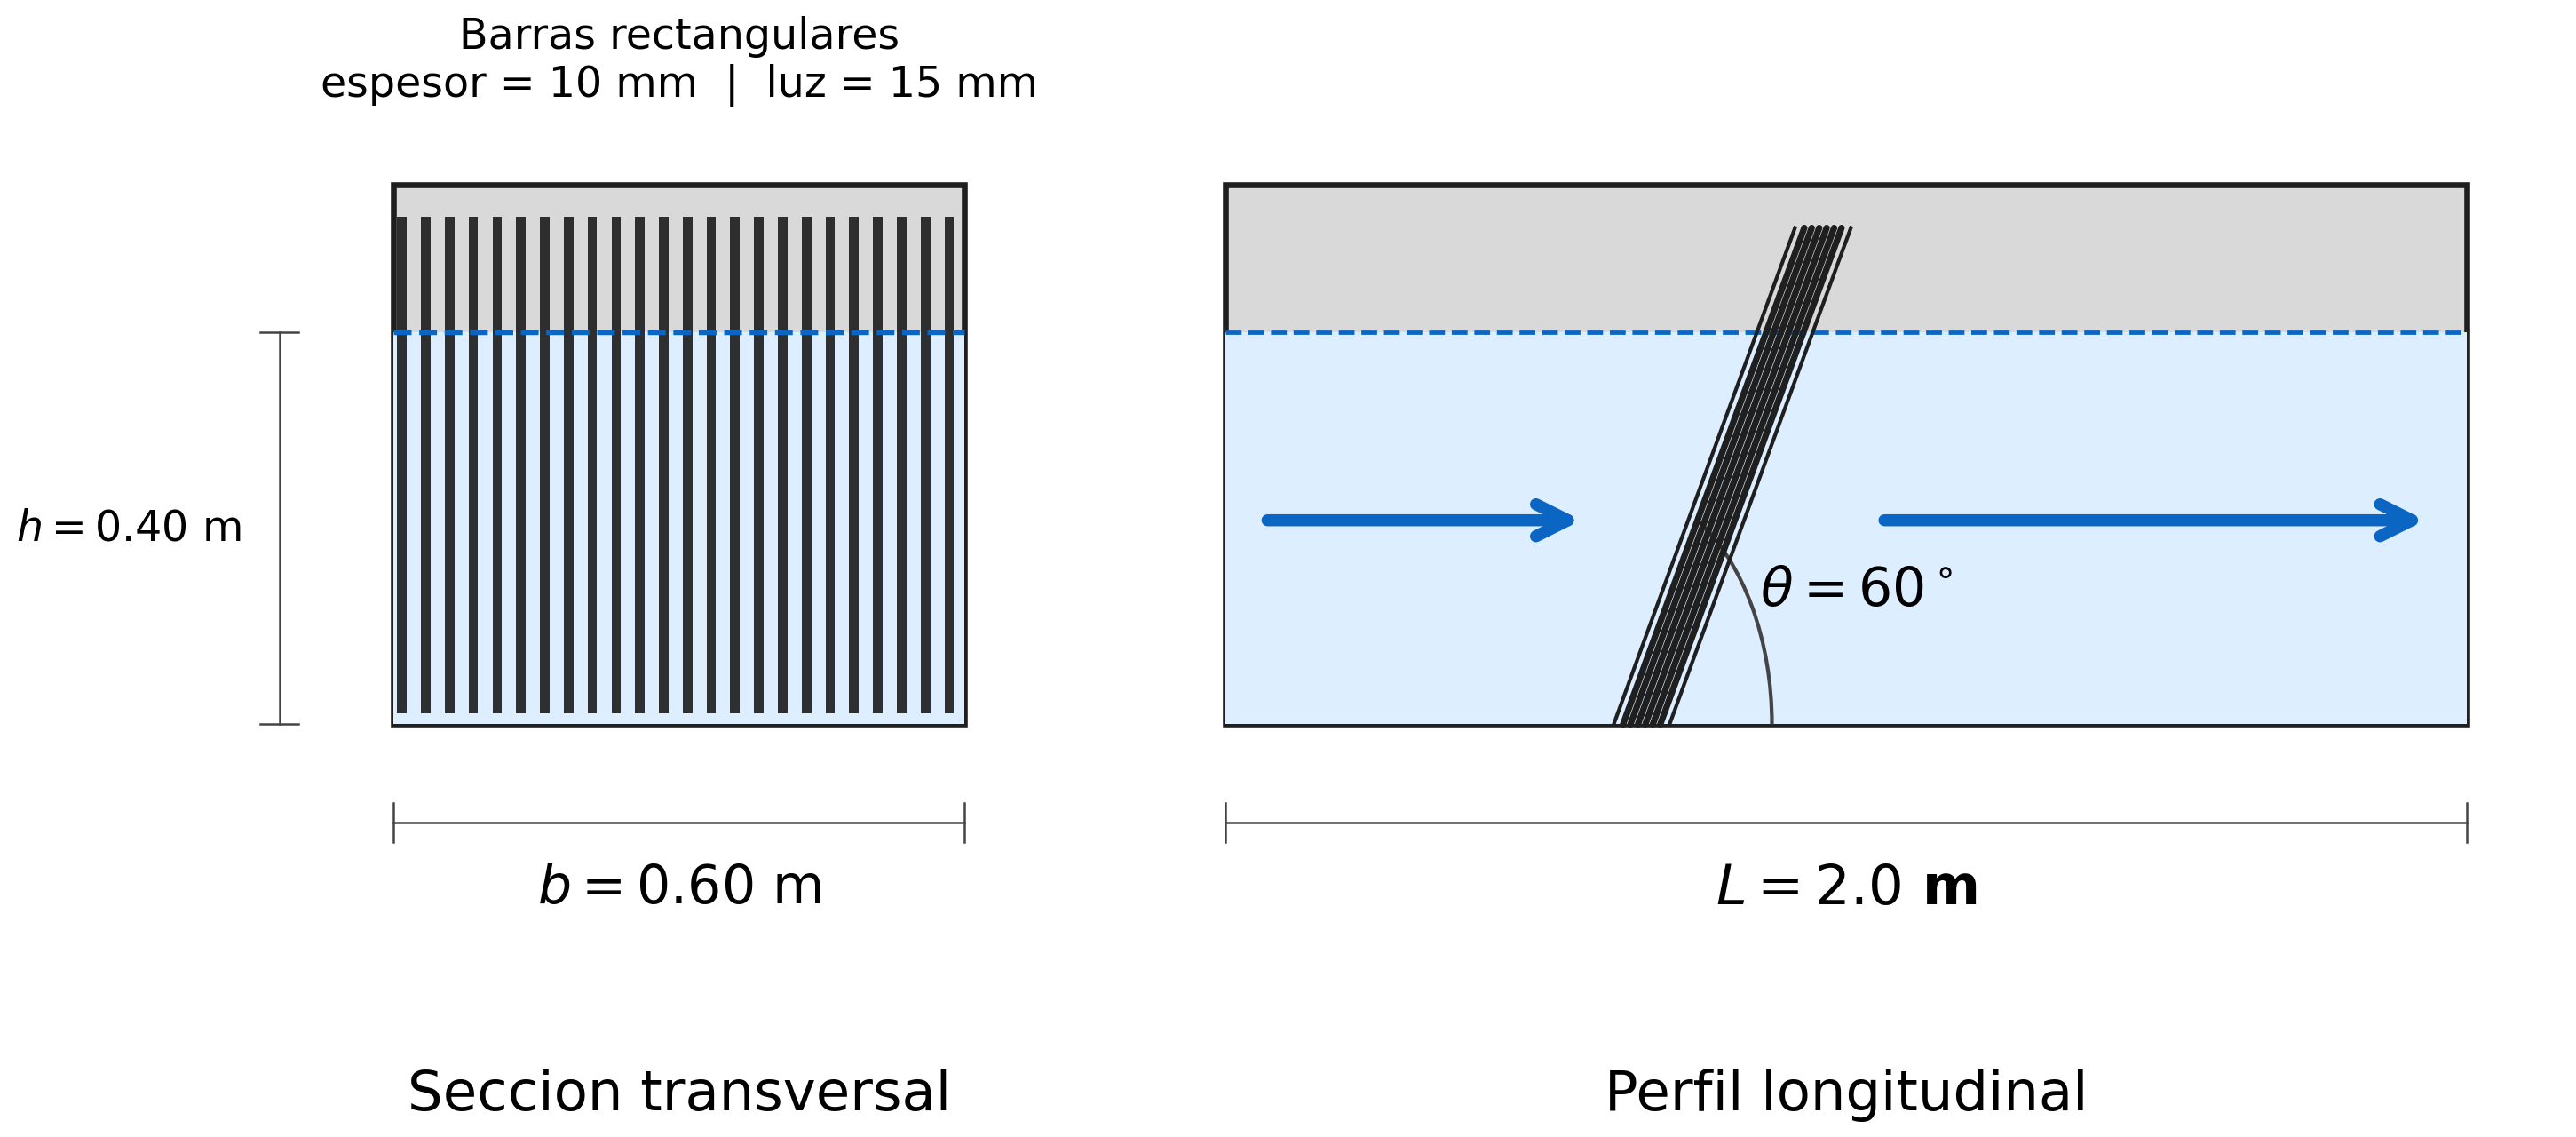
\includegraphics[width=0.9\textwidth]{figuras/rejillas_rejillas.png}
\caption{Esquema del canal de desbaste con rejillas (dimensiones en metros)}
\label{fig:rejillas}
\end{figure}





\textit{Nota sobre cantidades:} El presente dimensionamiento no estima la masa o volumen diario de residuos de cribado. Segun Metcalf y Eddy \cite{metcalf2014}, la produccion tipica de residuos de rejillas finas en aguas residuales municipales varia entre 0.005--0.02 m\textsuperscript{3}/1000 m\textsuperscript{3} de agua tratada. Para el caudal de diseno, esto representaria aproximadamente 0.02--0.09 m\textsuperscript{3}/d (total planta), sujeto a caracterizacion local.

Las dimensiones finales del canal con rejillas son: ancho 0.60 m, tirante 0.40 m y longitud 2.0 m. Se requieren dos unidades, una por cada linea de tratamiento.

\subsection{Desarenador de Flujo Horizontal}



El desarenador remueve part\'iculas minerales (arena, grava) con di\'ametro superior a 0.20~mm mediante sedimentaci\'on gravitacional. Seg\'un Metcalf y Eddy \cite{metcalf2014}, los par\'ametros de dise\~no son: velocidad horizontal 0.25--0.30~m/s (m\'aximo 0.30~m/s para evitar arrastre de sedimentos), tiempo de retenci\'on 30--60~s, y profundidad de flujo 0.75--2.0~m (OPS/CEPIS \cite{ops2005} permite valores menores en plantas peque\~nas).

La profundidad total del canal incluye: profundidad \'util de flujo (0.40~m), zona de almacenamiento de arena (0.25--0.30~m; se adopta 0.30~m), y bordo libre (0.30~m).

El dise\~no del desarenador se fundamenta en la teor\'ia de sedimentaci\'on discreta. Primero se calcula la velocidad de sedimentaci\'on de las part\'iculas objetivo mediante la Ley de Stokes:

\begin{equation}
v_s = \frac{g \cdot (S_s - 1) \cdot d^2}{18 \cdot \nu}
\end{equation}
\captionequation{Ley de Stokes - Velocidad de sedimentacion de particulas}

\textit{Donde:}
\begin{itemize}[noitemsep,leftmargin=2em]
    \item[$v_s$] = Velocidad de sedimentaci\'on (m/s)
    \item[$g$] = Aceleraci\'on de la gravedad (9.81 m/s²)
    \item[$S_s$] = Gravedad espec\'ifica de la arena (2.65)
    \item[$d$] = Di\'ametro de la part\'icula (0.00020 m)
    \item[$\nu$] = Viscosidad cinem\'atica del agua a 25.6°C ($8.3973e-07$ m²/s)
\end{itemize}

\begin{equation}
v_s = \frac{9.81 \times (2.65 - 1) \times (0.00020)^2}{18 \times 8.3973e-07} = 0.043 \text{ m/s}
\end{equation}

Con este valor de $v_s$ se determina la longitud te\'orica del desarenador mediante la ecuaci\'on de sedimentaci\'on tipo I:

\begin{equation}
L = \frac{H \cdot v_h}{v_s} = \frac{0.40 \times 0.30}{0.043} = 2.8 \text{ m}
\end{equation}

\textit{Donde:}
\begin{itemize}[noitemsep,leftmargin=2em]
    \item[$L$] = Longitud del desarenador (m)
    \item[$H$] = Profundidad \'util (0.40 m)
    \item[$v_h$] = Velocidad horizontal adoptada (0.30 m/s)
\end{itemize}

La longitud te\'orica resultante (2.8~m) es adecuada para el caudal de dise\~no y se adopta como longitud de dise\~no.

El ancho del canal se determina por la ecuaci\'on de continuidad:

\begin{equation}
B = \frac{Q}{v_h \cdot H} = \frac{0.00577}{0.30 \times 0.40} = 0.048 \text{ m}
\end{equation}

\textit{Donde:}
\begin{itemize}[noitemsep,leftmargin=2em]
    \item[$B$] = Ancho te\'orico del canal (m)
    \item[$Q$] = Caudal de dise\~no (0.00577 m³/s)
\end{itemize}

El ancho te\'orico resulta inferior al m\'inimo constructivo. Se adopta 0.60 m seg\'un OPS/CEPIS \cite{ops2005} y SENAGUA \cite{senagua2012}, que establecen 0.60 m como ancho m\'inimo para operaci\'on y mantenimiento.

Verificando la velocidad horizontal real con el ancho adoptado:

\begin{equation}
v_{real} = \frac{Q}{B \cdot H} = \frac{0.00577}{0.60 \times 0.40} = 0.024 \text{ m/s}
\end{equation}

El tiempo de retenci\'on real resulta:

\begin{equation}
t_r = \frac{L}{v_{real}} = \frac{3.0}{0.024} = 124.8 \text{ s}
\end{equation}

\subsubsection{Verificacion}

\textbf{Verificacion de Velocidad Critica de Resuspension}

Para garantizar que la arena sedimentada no sea resuspendida por el flujo, se verifica que la velocidad horizontal del dise\~no sea menor que la velocidad cr\'itica de resuspensi\'on, calculada mediante la f\'ormula de Camp-Shields:

\begin{equation}
v_c = \sqrt{\frac{8 \beta g (S_s - 1) d}{f}}
\end{equation}
\captionequation{Velocidad critica de resuspension - Camp-Shields}

\textit{Donde:}
\begin{itemize}[noitemsep,leftmargin=2em]
    \item[$v_c$] = Velocidad cr\'itica de resuspensi\'on (m/s)
    \item[$\beta$] = Factor de forma (0.05, rango 0.04--0.06)
    \item[$g$] = Aceleraci\'on de la gravedad (9.81 m/s²)
    \item[$S_s$] = Gravedad espec\'ifica de la arena (2.65)
    \item[$d$] = Di\'ametro de la part\'icula (0.00020 m)
    \item[$f$] = Factor de fricci\'on de Darcy-Weisbach (0.025, rango 0.02--0.03)
\end{itemize}

\begin{equation}
v_c = \sqrt{\frac{8 \times 0.05 \times 9.81 \times (2.65 - 1) \times 0.00020}{0.025}} = 0.228 \text{ m/s}
\end{equation}
\captionequation{Velocidad critica calculada}

\textbf{Verificacion para Caudal Maximo Horario}

Se verifica el comportamiento hidr\'aulico para el caudal m\'aximo horario, aplicando un factor de pico t\'ipico de 2.8 sobre el caudal medio:

\begin{equation}
Q_{max} = 2.8 \times Q_{medio} = 2.8 \times 5.8 = 16.0 \text{ L/s}
\end{equation}

A caudal m\'aximo, la velocidad horizontal resulta:

\begin{equation}
v_{h,max} = \frac{Q_{max}}{B \cdot H} = \frac{15.983/1000}{0.60 \times 0.40} = 0.067 \text{ m/s}
\end{equation}

El tiempo de retenci\'on a caudal m\'aximo:

\begin{equation}
t_{r,max} = \frac{L}{v_{h,max}} = \frac{3.0}{0.067} = 45.0 \text{ s}
\end{equation}

\textbf{Criterios de verificaci\'on de resuspensi\'on} (Camp-Shields, Metcalf y Eddy \cite{metcalf2014}):

La velocidad calculada $v_{h,max} = 0.067$~m/s se eval\'ua seg\'un (l\'imite: $v_c \times 90\% = 0.205$~m/s):

\begin{equation}
\text{Estado} = \begin{cases}
    \text{SEGURIDAD} & \text{si } v_{h,max} \leq 0.205 \text{ m/s} \quad \text{(no hay resuspensi\'on)} \\
    \text{RIESGO} & \text{si } v_{h,max} > 0.205 \text{ m/s} \quad \text{(arena resuspendida)}
\end{cases}
\end{equation}
\captionequation{Criterios de verificacion de resuspension}

Con la velocidad calculada $v_{h,max} = 0.067$~m/s, la unidad se clasifica como \textbf{SEGURIDAD}. En terminos de cumplimiento, la verificacion de resuspension \textbf{CUMPLE} porque es menor que el limite de resuspension con factor de seguridad (0.205~m/s), por lo que no se produce resuspension de la arena depositada.

\subsubsection{Resultados}

\begingroup
\small
\begin{longtable}{l p{9cm}}
\caption{Dimensiones del desarenador}\\
\toprule
Par\'ametro & Valor \\
\midrule
\endfirsthead
\caption[]{Dimensiones del desarenador (continuación)}\\
\toprule
Par\'ametro & Valor \\
\midrule
\endhead
\midrule
\multicolumn{2}{r}{\textit{Continúa en la siguiente página}} \\
\endfoot
\bottomrule
\endlastfoot
Longitud dise\~no & 3.0 m (m\'inimo constructivo SENAGUA) \\
Ancho & 0.60 m (m\'inimo constructivo) \\
Profundidad \'util & 0.40 m \\
Velocidad horizontal real & 0.024 m/s \\
Velocidad cr\'itica resuspensi\'on & 0.228 m/s (Camp-Shields) \\
Tiempo retenci\'on real & 124.8 s \\
\multicolumn{2}{p{\textwidth}}{\small\textit{$^a$Nota: El TRH de 125~s y velocidad de 0.024~m/s se deben al ancho m\'inimo constructivo de 0.60~m. }} \\
\end{longtable}
\endgroup

\textbf{Manejo de arena removida}

El desarenador retiene part\'iculas minerales, principalmente arena y grava fina, que se sedimentan en el fondo del canal por acci\'on gravitacional. Estas part\'iculas presentan di\'ametros superiores a 0.20~mm, con gravedad espec\'ifica de 2.65, correspondiendo a s\'olidos inorg\'anicos de alta densidad presentes en el agua residual. El canal incorpora una zona de almacenamiento de 0.30~m de altura, dimensionada espec\'ificamente para acumular la arena removida entre operaciones de limpieza. La frecuencia de limpieza recomendada es diaria o seg\'un la acumulaci\'on observada, manteniendo la arena acumulada por debajo del 50\% de la altura de almacenamiento designada para garantizar el funcionamiento \'optimo del sistema. La remoci\'on se realiza manualmente mediante palas y cubos desde la plataforma de operaci\'on, aunque puede implementarse un sistema de succi\'on o bombeo si el caudal y la producci\'on de arena lo justifican t\'ecnicamente.

\textbf{Disposici\'on final de la arena:}

La arena removida en el desarenador puede manejarse de diferentes formas seg\'un su composici\'on y la normativa local vigente. La opci\'on m\'as com\'un es el relleno sanitario, ya que la arena es material inorg\'anico inerte que puede disposicionarse en rellenos autorizados sin restricciones especiales. En caso de que la arena est\'e relativamente limpia, con bajo contenido de materia org\'anica adherida, existe la posibilidad de reuso condicionado para relleno y compactaci\'on en obras civiles previa caracterizaci\'on, mezcla con concreto para elementos no estructurales, o como complemento en sistemas de filtraci\'on gruesa previo lavado. Si se detecta alta carga org\'anica adherida a los granos de arena, evidenciada por olor f\'etido o color oscuro, se recomienda un lavado previo antes de la disposici\'on final para reducir el impacto ambiental.

\begin{figure}[H]
\centering

\includegraphics[width=\textwidth]{figuras/Esquema_Desarenador.png}
\caption{Esquema del desarenador de flujo horizontal con perfil longitudinal y corte transversal. Se muestran la entrada del afluente, la zona de flujo, el dep\'osito de arena y la salida . }
\label{fig:desarenador}
\end{figure}

\textit{Nota sobre cantidades:} El presente dimensionamiento no estima la masa o volumen diario de arena removida. Seg\'un Metcalf y Eddy \cite{metcalf2014}, la producci\'on t\'ipica de arena en aguas residuales municipales var\'ia entre 0.004--0.15 L/m\textsuperscript{3} de agua tratada, dependiendo de las caracter\'isticas del sistema de alcantarillado (red combinada vs. separada) y del suelo local. Para el caudal de dise\'no, esto representar\'ia aproximadamente 0.02--0.6 L/d (total planta), sujeto a caracterizaci\'on local.

\subsection{Reactor Anaerobio de Flujo Ascendente con Manto de Lodos (UASB)}



El reactor UASB (Upflow Anaerobic Sludge Blanket), desarrollado por Lettinga y colaboradores en 1980 en la Universidad de Wageningen de los Países Bajos \cite{vanhaandel1994}, es uno de los sistemas de tratamiento anaerobio de alta tasa más utilizados en el mundo para aguas residuales municipales y agroindustriales. El agua residual entra por la parte inferior y fluye en sentido ascendente a través de un manto denso de lodo anaerobio, donde los microorganismos anaerobios degradan la materia orgánica mediante metanogénesis, convirtiéndola en biogás (metano y CO$_2$) y biomasa. El proceso ocurre sin oxígeno molecular, por lo que no requiere aireación, reduciendo drásticamente el consumo energético (5--10 veces menos que un sistema aerobio convencional).

El diseño se fundamenta en criterios biológicos e hidráulicos establecidos por Van Haandel y Lettinga \cite{vanhaandel1994}, Sperling \cite{sperling2007} y Metcalf y Eddy \cite{metcalf2014}.

\textbf{Condiciones de temperatura:} La temperatura del agua residual es un factor crítico que determina los parámetros de diseño del reactor UASB. Según Van Haandel y Lettinga (1994), el proceso de metanogénesis requiere temperaturas superiores a 22°C para operar de manera óptima. A temperaturas menores, la actividad metabólica de los microorganismos anaerobios disminuye, requiriendo ajustes en la carga orgánica, el tiempo de retención y la velocidad ascendente.

Para el presente diseño, la temperatura del agua residual es \textbf{25.6°C} (óptima (>= 22°C)). Con base en esta condición, los parámetros de diseño se han ajustado automáticamente según los siguientes rangos recomendados:

\begin{table}[H]
\centering
\caption{Rangos de diseño según temperatura del agua residual}
\small
\begin{tabular}{lccc}
\toprule
\textbf{Condición} & \textbf{T (°C)} & \textbf{Cv (kg/m³·d)} & \textbf{HRT (h)} \\
\midrule
Óptima & $>=$ 22 & 2.0--3.0 & 4--6 \\
Moderada & 18--22 & 1.5--2.5 & 5--8 \\
Baja & 15--18 & 1.0--1.5 & 6--10 \\
Muy baja & 10--15 & 0.5--1.5 & 8--12 \\
Crítica & $<$ 10 & No recomendable & Requiere calefacción \\
\bottomrule
\end{tabular}
\end{table}

Para mantener el rendimiento óptimo del reactor en caso de descenso de temperatura, se recomienda monitorear periodicamente. Si la temperatura descendiera por debajo de 18°C, el sistema debería ajustar automáticamente la carga orgánica y el tiempo de retención.

Notas importantes de diseño: se debe incluir un separador gas-líquido-sólido (GLS) en la parte superior (altura referencial de 1.0 m) y un sistema de distribución uniforme en el fondo. El biogás requiere sistema de recolección y manejo seguro (prevención contra explosión).

Los siguientes parámetros han sido seleccionados como criterios de diseño para el reactor UASB:

\begin{table}[H]
\centering
\caption{Parámetros seleccionados para el diseño UASB}
\begin{tabular}{p{6cm}cc}
\toprule
\textbf{Parámetro} & \textbf{Valor adoptado} & \textbf{Rango recomendado} \\
\midrule
Caudal por línea ($Q$) & 20.77 m³/h & - \\
Carga orgánica volumétrica ($C_v$) & 2.50 kg DQO/m³·d & 2,0--3,0 \\
Velocidad ascendente de diseño ($v_{up}$) & 0.80 m/h & 0,5--1,5 \\
Altura máxima del reactor ($H_{max}$) & 6.0 m & 3.0--6.0 m \\
Factor de efectividad sedimentador & 90\% & 85--95\% \\
Altura sedimentador ($H_{sed}$) & 1.6 m & 1.5--2.0 m \\
Carga superficial máxima límite (SOR) & 1.2 m/h & $<$ 1.2 m/h \\
\bottomrule
\end{tabular}
\end{table}

\textit{Nota: El valor de velocidad ascendente indicado en el cuadro corresponde al parámetro de diseño configurado. Sin embargo, tras el proceso de verificación hidráulica según las condiciones de temperatura del agua residual (25.6°C) y los criterios de estabilidad del manto de lodos, el valor efectivo adoptado para el cálculo del área superficial es 0.39 m/h, resultando en un área de 53.45 m².}

\textbf{Zona de Reacción -- Dimensionamiento}

El dimensionamiento del reactor UASB se fundamenta en dos criterios complementarios: el criterio biológico (carga orgánica volumétrica) y el criterio hidráulico (velocidad ascendente). Ambos enfoques deben satisfacerse simultáneamente para garantizar el correcto funcionamiento del sistema.

\textbf{Criterio biológico:} Según Van Haandel y Lettinga \cite{vanhaandel1994}, el volumen del reactor se determina a partir de la carga orgánica volumétrica ($C_v$), que representa la cantidad de materia orgánica que debe procesar el reactor por unidad de volumen y tiempo. Para aguas residuales municipales a temperaturas superiores a 22°C, los autores recomiendan una carga entre 2.0 y 3.0 kg DQO/m³·d. La expresión fundamental es:

\begin{equation}
V_r = \frac{Q \cdot S_0}{C_v}
\end{equation}
\captionequation{Volumen util del reactor UASB segun Van Haandel y Lettinga (1994)}

\textit{Donde:}
\begin{itemize}[noitemsep,leftmargin=2em]
    \item[$V_r$] = Volumen útil del reactor (m³)
    \item[$Q$] = Caudal diario (498.5 m³/d)
    \item[$S_0$] = Concentración de DQO afluente (0.4980 kg/m³)
    \item[$C_v$] = Carga orgánica volumétrica adoptada (2.5 kg DQO/m³·d)
\end{itemize}

Sustituyendo los valores del proyecto:

\begin{equation}
V_{biol} = \frac{498.5 \times 0.4980}{2.5} = 99.3 \text{ m}^3
\end{equation}

Este volumen biológico teórico de 99.3 m³ garantizaría el tiempo de retención hidráulico necesario para que los microorganismos anaerobios degraden la materia orgánica según Van Haandel y Lettinga. Sin embargo, el criterio hidráulico (velocidad ascendente) requiere un área superficial mayor para evitar el arrastre del manto de lodos, lo que resulta en un volumen final adoptado de \textbf{160.4 m³}. Este ajuste incrementa el TRH respecto al mínimo teórico, proporcionando un margen de seguridad adicional en la operación del reactor.

\textbf{Criterio hidráulico:} De manera simultánea, según Sperling \cite{sperling2007}, la velocidad ascendente ($v_{up}$) debe mantenerse dentro de rangos que permitan retener el manto de lodos sin arrastre. El autor recomienda velocidades entre 0.5 y 1.5 m/h para condiciones normales, con un máximo de 2.0 m/h durante picos de caudal. Con la velocidad adoptada de 0.39 m/h, el área superficial requerida se calcula como:

\begin{equation}
A_s = \frac{Q}{v_{up}}
\end{equation}
\captionequation{Area superficial del reactor UASB}

\textit{Donde:}
\begin{itemize}[noitemsep,leftmargin=2em]
    \item[$A_s$] = Área superficial del reactor (m²)
    \item[$Q$] = Caudal por línea (20.77 m³/h)
    \item[$v_{up}$] = Velocidad ascendente adoptada (0.39 m/h)
\end{itemize}

\begin{equation}
A_s = \frac{20.77}{0.39} = 53.45 \text{ m}^2
\end{equation}

El diámetro del reactor circular se obtiene a partir de la geometría del círculo, considerando que el área superficial debe ser la calculada hidráulicamente. Esta formulación geométrica estándar permite determinar las dimensiones constructivas del reactor:

\begin{equation}
D = \sqrt{\frac{4 \cdot A_s}{\pi}}
\end{equation}
\captionequation{Diametro del reactor circular - Geometria basica}

\textit{Donde:}
\begin{itemize}[noitemsep,leftmargin=2em]
    \item[$D$] = Diámetro del reactor circular (m)
    \item[$A_s$] = Área superficial calculada (53.45 m²)
    \item[$\pi$] = 3,14159
\end{itemize}

\begin{equation}
D = \sqrt{\frac{4 \times 53.45}{\pi}} = 8.25 \text{ m}
\end{equation}

La altura de la zona de reacción (manto de lodos) resulta 3.00~m, proporcionando un tiempo de retención hidráulico de 7.7 horas para la temperatura de 25.6°C del agua residual. La evaluación de adecuación hidráulica se presenta en la sección de verificación.

\textbf{Producción de biogás:} La metanogénesis en el reactor UASB genera biogás compuesto principalmente por metano (CH$_4$) y dióxido de carbono (CO$_2$). Según Van Haandel y Lettinga \cite{vanhaandel1994}, la producción teórica de metano puede estimarse mediante relaciones estequiométricas. Experimentalmente se ha determinado que por cada kilogramo de DQO removida en condiciones anaerobias, se producen aproximadamente 0,35 m³ de metano (a condiciones estándar). Esta relación permite estimar la producción esperada de biogás:

El biogás generado en reactores UASB tratando aguas residuales municipales está compuesto principalmente por metano (CH$_4$) en una proporción de 65\%, situándose típicamente en un rango de 60 a 75\%. El metano constituye el componente energético del biogás, con un poder calorífico de aproximadamente 35 MJ/m³. El dióxido de carbono (CO$_2$) representa alrededor del 35\% del volumen total, con un rango típico entre 25 y 40\%, siendo un producto natural de la digestión anaerobia. El sulfuro de hidrógeno (H$_2$S) se presenta en concentraciones inferiores a 100 ppm, proveniente de la reducción de sulfatos presentes en el agua residual; cuando las concentraciones son elevadas se requiere tratamiento debido a su corrosividad y generación de olores. Finalmente, el biogás contiene vapor de agua y trazas de nitrógeno, oxígeno y otros gases en proporciones menores al 1\%.

El biogás producido debe manejarse de manera segura considerando aspectos de seguridad, aprovechamiento y monitoreo. En cuanto a seguridad, el biogás es inflamable en concentraciones del 5 al 15\% en aire, por lo que se requiere un sistema de venteo o quemador para evitar su acumulación. Respecto al aprovechamiento, existen tres opciones principales: el quemador de antorcha para eliminación segura, el calentamiento del propio reactor cuando la temperatura lo requiere, y la generación de energía eléctrica mediante microturbinas, aunque esta última requiere una evaluación de viabilidad económica. El monitoreo debe incluir el control periódico de la composición del biogás, especialmente el contenido de H$_2$S, así como la verificación del sistema de sellado del reactor.

El proceso de metanogénesis es sensible a las condiciones de pH, por lo que según Van Haandel y Lettinga \cite{vanhaandel1994} y Metcalf y Eddy \cite{metcalf2014} es necesario mantener rangos óptimos de operación. El pH óptimo debe situarse entre 6.8 y 7.2, ya que valores por debajo de 6,5 inhiben la actividad metanogénica y pueden causar la acidificación del reactor. Respecto a la alcalinidad, se recomienda un mínimo de 1000 mg/L como CaCO$_3$, ya que actúa como tampón ante la producción de ácidos durante la digestión, manteniendo la estabilidad del pH.

\textit{Nota:} Las aguas residuales municipales típicamente contienen suficiente alcalinidad (bicarbonatos) para mantener el pH estable durante la digestión anaerobia. Si el pH del efluente descendiera consistentemente por debajo de 6,8, se debería evaluar la adición de fuentes de alcalinidad (carbonato cálcico, hidróxido de sodio) o revisar la carga orgánica aplicada.

El lodo producido en el reactor UASB está estabilizado anaeróbicamente. Durante su retención prolongada en el reactor, donde el tiempo de retención de sólidos es significativamente mayor que el tiempo de retención hidráulico, los microorganismos completan las etapas de digestión: hidrólisis, acidogénesis, acetogénesis y metanogénesis. Como resultado, el lodo estabilizado presenta bajo contenido de materia orgánica volátil, con una reducción de 40 a 60\% respecto al lodo primario no estabilizado, ausencia de olores fétidos característicos de lodos frescos, mayor facilidad de deshidratación en lechos de secado, y una reducción significativa de patógenos, aunque sin alcanzar la esterilización completa.

Esta estabilización hace que el lodo UASB sea más manejable para disposición final o uso condicionado en agricultura, comparado con lodos de tratamientos aerobios o sedimentación primaria sin digestión.

\begin{equation}
V_{CH_4} = (Q_d \cdot S_0 \cdot E) \times 0.35
\end{equation}
\captionequation{Produccion de biogas - Relacion estequiometrica}

\textit{Donde:}
\begin{itemize}[noitemsep,leftmargin=2em]
    \item[$V_{CH_4}$] = Volumen de metano producido (m³ CH$_4$/d)
    \item[$Q_d$] = Caudal diario (498.5 m³/d)
    \item[$S_0$] = Concentración de DQO afluente (0.498 kg/m³)
    \item[$E$] = Eficiencia de remoción (0.65)
\end{itemize}

\begin{equation}
V_{CH_4} = (498.5 \times 0.498 \times 0.65) \times 0.35 = 56.5 \text{ m}^3 \text{ CH}_4\text{/d}
\end{equation}

\textbf{Cámara de Sedimentación -- Dimensionamiento}

El compartimiento de sedimentación superior constituye una zona crítica del reactor UASB, ya que debe retener los sólidos biológicos antes de que salgan con el efluente. Según Chernicharo \cite{chernicharo2007}, el diseño de esta zona se fundamenta en el concepto de Carga Superficial (SOR - Surface Overflow Rate), análogo al utilizado en sedimentadores convencionales, pero adaptado a las condiciones particulares del UASB donde el biogás generado puede afectar la sedimentación.

Chernicharo recomienda que la carga superficial a caudal máximo no debe exceder 1.2 m/h para evitar el arrastre de sólidos hacia el efluente. Este valor es más restrictivo que el utilizado en sedimentadores primarios convencionales debido a la presencia de biogás y la naturaleza floculenta de los lodos anaerobios. Adicionalmente, el autor sugiere una altura mínima del compartimiento de sedimentación entre 1.5 y 2.0 m para garantizar el tiempo necesario de separación gas-líquido-sólido.

Los criterios de diseño según Chernicharo (2007) son:

\begin{equation}
\text{SOR}_{max} < 1.2 \text{ m/h} \quad \text{(límite para evitar arrastre de sólidos)}
\end{equation}

\begin{equation}
H_{sed} \geq 1.5 \text{ m} \quad \text{(altura mínima constructiva)}
\end{equation}

El área efectiva de sedimentación considera el factor de efectividad del 90\% del área total (Chernicharo):

\begin{equation}
A_{sed} = 0.90 \times A_{sup} = 0.90 \times 53.45 = 48.11 \text{ m}^2
\end{equation}

El volumen del sedimentador se calcula con la altura adoptada de 1.6~m:

\begin{equation}
V_{sed} = A_{sed} \times H_{sed} = 48.11 \times 1.6 = 76.97 \text{ m}^3
\end{equation}

El tiempo de retención hidráulico en el sedimentador resulta:

\begin{equation}
t_{sed} = \frac{V_{sed}}{Q} = \frac{76.97}{20.77} = 3.71 \text{ h}
\end{equation}

\textbf{Aberturas GLS -- Dimensionamiento}

El separador gas-líquido-sólido (GLS) incluye aberturas que permiten el paso del líquido clarificado desde la zona de digestión hacia el compartimiento de sedimentación. Según Chernicharo \cite{chernicharo2007}, estas aberturas deben dimensionarse cuidadosamente para evitar velocidades que arrastren sólidos hacia el efluente.

La velocidad admisible en las aberturas es mayor que en el cuerpo del reactor porque el líquido ya está parcialmente clarificado. Los valores recomendados son 2.0--2.3 m/h a caudal medio y hasta 4.2 m/h a caudal máximo. El área mínima requerida se calcula como:

\begin{equation}
A_{ab} = \frac{Q}{v_{adm}}
\end{equation}
\captionequation{Area minima de aberturas GLS}

\textit{Donde:}
\begin{itemize}[noitemsep,leftmargin=2em]
    \item[$A_{ab}$] = Área total libre de aberturas (m²)
    \item[$Q$] = Caudal por línea (20.77 m³/h)
    \item[$v_{adm}$] = Velocidad admisible adoptada (1.52 m/h)
\end{itemize}

\begin{equation}
A_{ab} = \frac{20.77}{1.52} = 13.70 \text{ m}^2
\end{equation}

Adicionalmente, el GLS debe construirse con pendientes de 50° a 60° (adoptado 55°) y un traslape de 0.15 m sobre las aberturas para garantizar la retención de sólidos.

\textbf{Distribución del Afluente -- Dimensionamiento}

La distribución uniforme del afluente en el fondo del reactor es crítica para garantizar un flujo ascendente homogéneo y evitar cortocircuitos que reducirían la eficiencia del tratamiento. Según Chernicharo \cite{chernicharo2007}, el número de puntos de distribución se determina en función del área del reactor y el área de influencia que puede atender cada punto.

El área de influencia por punto recomendada varía entre 2.0 y 3.0 m² por punto. Adoptando un valor intermedio de 2.50 m²/punto, el número de puntos de distribución resulta:

\begin{equation}
N = \frac{A}{A_{inf}} = \frac{53.45}{2.50} = 22 \text{ puntos}
\end{equation}
\captionequation{Numero de puntos de distribucion del afluente}

El caudal por punto de distribución se calcula dividiendo el caudal total entre el número de puntos:

\begin{equation}
q = \frac{Q}{N} = \frac{0.006 \times 1000}{22} = 0.262 \text{ L/s}
\end{equation}

Los tubos de distribución se diseñan según la práctica estándar de Lettinga y Hulshoff Pol: tubería principal de gran diámetro para transporte sin obstrucciones, con bocas de salida reducidas para garantizar velocidad de inyección adecuada. Se adopta una tubería de distribución de 50 mm con bocas de salida de 25 mm.

\textbf{Verificación de velocidades:}

La velocidad en la tubería principal(transporte) se calcula como:

\begin{equation}
v_{tubo} = \frac{q}{a_{tubo}} = \frac{0.262 \times 10^{-3}}{\pi \times (50 \times 10^{-3})^2 / 4} = 0.134 \text{ m/s}
\end{equation}

La velocidad en la boca de salida (inyección al lecho de lodo) es el parámetro crítico según Lettinga. Debe estar entre 0.4 y 4.0 m/s para garantizar arrastre de sólidos sin erosión:

\begin{equation}
v_{boca} = \frac{q}{a_{boca}} = \frac{0.262 \times 10^{-3}}{\pi \times (25 \times 10^{-3})^2 / 4} = 0.53 \text{ m/s}
\end{equation}

\subsubsection{Verificación}

\textbf{Verificación de Velocidad Ascendente a Caudal Máximo}

El fundamento de la verificación hidráulica establece que el diseño del reactor UASB debe garantizar no solo el funcionamiento adecuado bajo condiciones normales (caudal medio), sino también durante eventos de pico de caudal que ocurren típicamente en horas de mayor consumo de agua. Según Metcalf y Eddy \cite{metcalf2014}, los sistemas de tratamiento deben verificarse para el caudal máximo horario, el cual se estima aplicando un factor de pico sobre el caudal medio diario. El factor denominado $f_p$, adoptado de 2.8 considera las características de la zona de estudio y las variaciones esperadas del caudal durante el día. La aplicación de este factor permite determinar el caudal máximo horario de diseño:

\begin{equation}
Q_{max} = f_p \times Q_{medio} = 2.8 \times 498.5 = 1380.9 \text{ m}^3\text{/d} = 57.54 \text{ m}^3\text{/h}
\end{equation}

El análisis de la velocidad ascendente de pico considera que, bajo condiciones de caudal máximo, la velocidad ascendente en el reactor aumenta proporcionalmente. Esta velocidad de pico, $v_{up,max}$, se calcula manteniendo el área superficial del reactor (determinada previamente por el criterio de velocidad media) pero incrementando el caudal al valor máximo esperado:

\begin{equation}
v_{up,max} = \frac{Q_{max}}{A_s} = \frac{57.54}{53.45} = 1.08 \text{ m/h}
\end{equation}

Los criterios de evaluación del estado del reactor, según Metcalf y Eddy \cite{metcalf2014}, clasifican el estado operacional en función de la velocidad ascendente máxima calculada. Esta clasificación permite determinar si el diseño garantiza la estabilidad del manto de lodos o si existe riesgo de arrastre de biomasa. Los autores definen tres estados operacionales basados en estudios experimentales de la hidrodinámica de reactores UASB. Formalmente, el estado se determina mediante:

\begin{equation}
\text{Estado} = \begin{cases}
    \text{ÓPTIMO} & \text{si } v_{up,max} \leq 1.5 \text{ m/h} \\
    \text{ACEPTABLE} & \text{si } 1.5 < v_{up,max} \leq 2.0 \text{ m/h} \\
    \text{NO ADMISIBLE} & \text{si } v_{up,max} > 2.0 \text{ m/h}
\end{cases}
\end{equation}
\captionequation{Criterios de verificación de arrastre del manto según Metcalf y Eddy (2014)}

Para el presente diseño, con una velocidad ascendente máxima calculada de $v_{up,max} = 1.08$~m/h, el reactor se clasifica en estado \textbf{ÓPTIMO}. Este resultado indica que el dimensionamiento propuesto requiere monitoreo durante eventos de pico de caudal.

\textbf{Verificación de la Cámara de Sedimentación}

El principio de verificación de la sedimentación establece que la cámara de sedimentación superior del reactor UASB debe evaluarse tanto para condiciones de caudal medio como para caudal máximo. Según Chernicharo \cite{chernicharo2007}, la verificación a caudal medio permite evaluar si el diseño opera dentro del rango óptimo de eficiencia, mientras que la verificación a caudal máximo determina si se evita el arrastre de sólidos durante picos de flujo.

El autor establece que, aunque el criterio crítico es el SOR máximo ($<$ 1.2 m/h), también es deseable que el SOR medio se mantenga entre 0.6 y 0.8 m/h. Valores inferiores a este rango, aunque conservadores, indican que el área del sedimentador es mayor de lo estrictamente necesario, lo cual no representa un problema operativo pero implica mayores costos de construcción. Valores superiores sugieren riesgo de arrastre incluso en operación normal.

El cálculo de la Carga Superficial Operacional se realiza aplicando la ecuación fundamental del SOR para ambas condiciones de caudal:

Para caudal medio (condición de operación normal):
\begin{equation}
SOR_{medio} = \frac{Q_{medio}}{A_{sed}} = \frac{20.77}{48.11} = 0.43 \text{ m/h}
\end{equation}

Para caudal máximo horario (condición de pico):
\begin{equation}
SOR_{max} = \frac{Q_{max}}{A_{sed}} = \frac{57.54}{48.11} = 1.20 \text{ m/h}
\end{equation}

El análisis de cumplimiento de criterios evalúa los valores calculados según los parámetros establecidos por Chernicharo (2007) para sedimentadores en reactores UASB:


     \textbf{SOR máximo}: La carga superficial máxima de 1.20 m/h cumple con el límite (< 1.2 m/h). Este límite representa la velocidad de asentamiento mínima de los agregados de lodos anaerobios. Superar este valor implica que el flujo ascendente supera la velocidad de caída de los sólidos, causando su arrastre hacia el efluente.
    
     \textbf{SOR medio}: La carga superficial de 0.43 m/h está por debajo del rango (0.6-0.8 m/h), pero es aceptable para diseño conservador. Según Chernicharo, este rango permite evaluar la eficiencia de separación sólido-líquido y el margen operativo de la cámara de sedimentación.
    
     \textbf{TRH en sedimentador}: El tiempo de retencion de 3.71 h cumple con el minimo de 1.5 h recomendado por Chernicharo para permitir la adecuada separacion gas-liquido-solido.


\begin{table}[H]
\centering
\caption{Verificación de criterios de diseño de la cámara de sedimentación según Chernicharo (2007)}
\begin{tabular}{lccc}
\toprule
\textbf{Parámetro} & \textbf{Valor calculado} & \textbf{Criterio} & \textbf{Estado} \\
\midrule
SOR máximo & 1.20 m/h & $<$ 1.2 m/h & Cumple \\
SOR medio & 0.43 m/h & 0.6--0.8 m/h & Bajo (aceptable) \\
TRH sedimentador & 3.71 h & $\geq$ 1.5 h & Cumple \\
\bottomrule
\end{tabular}
\end{table}

\textbf{Nota sobre márgenes operativos:} Los parámetros críticos de control hidráulico del reactor se mantienen dentro de los límites recomendados por Chernicharo \cite{chernicharo2007}. El SOR máximo es 1.20 m/h frente al límite de 1.2 m/h, con un margen de 0.3%; este criterio controla el riesgo de arrastre de sólidos en la cámara de sedimentación durante caudales pico. La velocidad máxima en aberturas GLS es 4.20 m/h frente al límite de 4.2 m/h, con un margen de 0.0%; este criterio controla el paso del líquido clarificado hacia el compartimiento de sedimentación sin inducir arrastre de lodos. En conjunto, el margen operativo se clasifica como reducido. Por ello, aunque la unidad cumple, se recomienda verificar SOR y velocidad en aberturas durante la puesta en marcha y monitorear periódicamente SST/turbidez del efluente como indicador de posible arrastre.

La verificacion muestra que el SOR medio esta por debajo del rango optimo pero dentro de valores aceptables conservadores; el diseno cumple con SOR maximo y TRH.

\textbf{Verificación de Aberturas GLS}

Verificando para caudal máximo ($Q_{max} = 57.54$ m³/h):

\begin{equation}
v_{ab,max} = \frac{Q_{max}}{A_{ab}} = \frac{57.54}{13.70} = 4.20 \text{ m/h} \quad \leq 4.2 \text{ m/h } \text{(Cumple)}
\end{equation}

La velocidad máxima calculada en las aberturas GLS es 4.20 m/h, menor o igual al límite de 4.2 m/h recomendado para caudal máximo. Esta condición indica que el área libre adoptada permite el paso del líquido clarificado hacia la cámara de sedimentación sin imponer velocidades que favorezcan el arrastre de sólidos del manto de lodos. En términos operativos, las aberturas funcionan como zona de transición hidráulica entre la digestión y la sedimentación; por ello se recomienda mantener limpias las ranuras del GLS y verificar su condición durante inspecciones de rutina.

\textbf{Verificación del Sistema de Distribución}

\begin{table}[H]
\centering
\caption{Verificación de velocidades en sistema de distribución}
\begin{tabular}{lccc}
\toprule
\textbf{Parámetro} & \textbf{Valor} & \textbf{Criterio} & \textbf{Estado} \\
\midrule
Velocidad en tubería principal& 0.134 m/s & Transporte sin obstrucción ($<$ 0.20 m/s) & Adecuado \\
Velocidad en boca de salida & 0.53 m/s & 0.4--4.0 m/s & Cumple \\
\bottomrule
\end{tabular}
\end{table}

La velocidad en boca de 0.53 m/s cumple con el rango recomendado por Lettinga y Hulshoff Pol para inyeccion adecuada en el lecho de lodo.

\subsubsection{Resultados}

\begingroup
\small
\begin{longtable}{ll}
\caption{Dimensiones y parámetros del reactor UASB}\\
\toprule
Parámetro & Valor \\
\midrule
\endfirsthead
\caption[]{Dimensiones y parámetros del reactor UASB (continuación)}\\
\toprule
Parámetro & Valor \\
\midrule
\endhead
\midrule
\multicolumn{2}{r}{\textit{Continúa en la siguiente página}} \\
\endfoot
\bottomrule
\endlastfoot
Diámetro & 8.25 m \\
\multicolumn{2}{l}{\textit{Desglose de alturas:}} \\
\quad Zona de distribución (fondo) & 0.30 m \\
\quad Zona de reacción (manto de lodos) & 3.00 m \\
\quad Zona de sedimentación & 1.60 m \\
\quad Separador GLS & 1.00 m \\
\quad Bordo libre & 0.50 m \\
\midrule
\textbf{Altura total de construcción} & \textbf{6.40 m} \\
\midrule
Volumen útil & 160.4 m³ \\
Área superficial & 53.45 m² \\
Tiempo de retención hidráulico & 7.7 h \\
Carga orgánica volumétrica & 2.5 kg DQO/m³·d \\
Biogás producido & 56.5 m$^3$ CH$_4$/d \\
\midrule
\multicolumn{2}{l}{\textit{Subdivisión zona de reacción:}} \\
\quad Lecho de lodo denso/granular (40\%) & 1.20 m \\
\quad Manto expandido (60\%) & 1.80 m \\
\end{longtable}
\endgroup

La subdivisión interna de la zona de reacción sigue criterios establecidos por Chernicharo \cite{chernicharo2007}. El lecho de lodo denso o granular (aproximadamente 40\% de la altura útil) contiene los lodos más viejos y densos, mientras que el manto de lodos expandido (aproximadamente 60\% de la altura útil) mantiene los lodos en suspensión activa donde ocurre la mayor parte de la degradación biológica.

El reactor UASB requiere un inóculo inicial de lodo anaeróbico denso/granular o, en su defecto, lodo digerido anaeróbicamente. Según Lettinga y Hulshoff-Pol \cite{vanhaandel1994}, la cantidad recomendada de inóculo para el arranque es de 10--15 kg SSV/m³ (sólidos suspendidos volátiles), equivalente a llenar aproximadamente el 15--30\% del volumen del reactor. El lodo granular consiste en agregados microbianos densos de 0.5--5 mm de diámetro, con velocidades de sedimentación superiores a 50 m/h. Si no se dispone de lodo granular, pueden utilizarse alternativas como lodo de digestor anaerobio, estiércol de cerdo/vaca o lodo de fosas sépticas, desarrollándose la granulación natural en un período de 2--6 meses mediante aumento gradual de la carga orgánica. 


La siguiente figura presenta un esquema del reactor UASB con sus componentes principales y los flujos de agua y biogás:

\begin{figure}[H]
\centering

\includegraphics[width=\textwidth]{figuras/Esquema_UASB.png}
\caption{Esquema del reactor UASB: distribución del afluente, zonas de reacción, separación gas-líquido-sólido y recolección de biogás. Caudal por línea: 20.77 m³/h, Biogás: 56.5 m³ CH$_4$/d, 22 puntos de distribución.}
\label{fig:esquema_uasb}
\end{figure}

El esquema ilustra el flujo ascendente del afluente a través del lecho de lodo denso, donde ocurre la digestión anaerobia. El biogás producido se separa en el GLS y se recolecta en la cámara superior, mientras que el efluente tratado sale por el lateral del reactor. La velocidad ascendente de diseño de 0.39 m/h garantiza la retención del manto de lodos.

\subsection{Filtro Percolador}

\subsubsection{Dimensionamiento}

El filtro percolador (también denominado trickling filter) constituye la unidad de tratamiento secundario aerobio por biopelícula (attached growth), diseñada específicamente para remover la carga orgánica restante después del tratamiento anaerobio en el UASB. Este reactor biológico opera mediante el paso del agua residual por gravedad a través de un medio poroso, donde se desarrolla una biopelícula aerobia (biofilm) de aproximadamente 0.1--0.2 mm de espesor que adsorbe y oxida la materia orgánica.

El principio de funcionamiento se basa en el contacto intermitente entre el agua residual, la biopelícula y el aire, permitiendo la degradación aerobia de la DBO. El aire circula por convección natural en sentido contrario (o igual, según la temperatura) al flujo del agua, suministrando el oxígeno necesario para mantener la actividad microbiana. Los microorganismos forman una capa adherida al medio denominada biopelícula, mientras que el exceso de biomasa (sloughings) se desprende periódicamente y es recolectado en el sistema de drenaje inferior (underdrain), requiriendo posterior sedimentación secundaria.

El dimensionamiento del filtro percolador se realiza mediante el criterio de carga orgánica volumétrica (COV) según WEF MOP-8 (2010), que es el método estándar para el diseño de filtros con medio plástico. Este enfoque garantiza que el volumen de medio sea suficiente para soportar la carga biológica aplicada sin riesgo de sobrecarga orgánica.

El modelo cinético de Germain (1966) se utiliza como verificación complementaria para estimar la concentración de DBO en el efluente y confirmar que el diseño cumple con el objetivo de calidad del agua tratada. Este modelo describe la remoción de DBO mediante una expresión exponencial relacionada con la profundidad del medio y la tasa hidráulica aplicada.



Según Metcalf \& Eddy (2014), existen tres tipos principales de medio filtrante, con el plástico aleatorio siendo la opción recomendada para plantas post-UASB debido a su menor peso, mayor profundidad posible y mejor aireación:

\begin{table}[H]
\centering
\caption{Comparación de tipos de medio filtrante (Metcalf \& Eddy, 2014)}
\small
\begin{tabular}{lccc}
\toprule
\textbf{Parámetro} & \textbf{Roca/Grava} & \textbf{Plástico Aleatorio} & \textbf{Plástico Estructurado} \\
\midrule
Superficie específica & 40--70 m²/m³ & 90--150 m²/m³ & 100--200 m²/m³ \\
Índice de vacíos & 40--50 \% & 94--97 \% & 95--99 \% \\
Densidad aparente & 800--1100 kg/m³ & 30--100 kg/m³ & 20--80 kg/m³ \\
Profundidad máxima & 1.5--3.0 m & 6--12 m & 6--15 m \\
Carga orgánica máxima & 0.08--0.32 kg/m³·d & 0.3--3.0 kg/m³·d & 0.5--5.0 kg/m³·d \\
\bottomrule
\end{tabular}
\end{table}

\textbf{Nota importante:} Para tratamiento carbonáceo (solo DBO, sin nitrificación) con medio plástico, la superficie específica no debe exceder 100 m²/m³ para evitar taponamiento por biopelícula excesiva (WEF, Manual of Practice No. 8).

\textbf{Parámetros de diseño}

\begin{table}[H]
\centering
\caption{Parámetros de diseño para filtro percolador}
\begin{tabular}{lccc}
\toprule
\textbf{Parámetro} & \textbf{Rango} & \textbf{Valor adoptado} & \textbf{Fuente} \\
\midrule
Carga orgánica (kg DBO/m³·d) & 0.3--3.0 & 0.33 & WEF MOP-8 \\
Profundidad medio (m) & 3.0--8.0 & 3.50 & Metcalf \& Eddy \\
Espacio distribuidor--medio (m) & 0.15--0.23 & 0.20 & EPA (2000) \\
Altura underdrain (m) & 0.45--0.60 & 0.50 & Metcalf \& Eddy \\
Bordo libre (m) & 0.30--0.50 & 0.30 & Norma constructiva \\
Recirculación R (-) & 0.5--2.0 & 1.0 & Metcalf \& Eddy \\
\bottomrule
\end{tabular}
\end{table}

\textbf{Carga Orgánica -- Dimensionamiento}

Según las recomendaciones para medio plástico aleatorio, las cargas óptimas oscilan entre 0.3 y 3.0 kg DBO/m³·d. Se adopta un valor conservador de 0.33 kg DBO/m³·d, apropiado para la condición de pretratamiento previo con UASB.

El volumen de medio filtrante requerido se calcula mediante:

\begin{equation}
V = \frac{Q \cdot S_0}{C_v}
\end{equation}
\captionequation{Volumen de medio filtrante - Filtro Percolador}

\textit{Donde:}
\begin{itemize}[noitemsep,leftmargin=2em]
    \item[$V$] = Volumen de medio filtrante requerido (m³)
    \item[$Q$] = Caudal diario (498.5 m³/d)
    \item[$S_0$] = DBO afluente (69 mg/L = 69 $\times$ 10$^{-3}$ kg/m³)
    \item[$C_v$] = Carga orgánica volumétrica (0.33 kg DBO/m³·d)
\end{itemize}

\begin{equation}
V = \frac{498.5 \times 69 \times 10^{-3}}{0.33} = 104.1 \text{ m}^3
\end{equation}

Con una profundidad de medio de 3.50 m, el área superficial resulta 29.75 m², correspondiendo a un diámetro de 6.15 m para configuración circular. La altura total incluye zonas de distribución (0.20 m), recolección (0.50 m) y bordo libre (0.30 m), resultando en 4.50 m.

El sistema incorpora recirculación con relación $R = 1.0$, lo cual mejora la distribución hidráulica y mantiene la biopelícula húmeda. La tasa hidráulica aplicada resulta 1.396 m³/m²·h.

\textbf{Recirculación -- Dimensionamiento}

La recirculación en filtros percoladores cumple funciones fundamentales según Metcalf \& Eddy \cite{metcalf2014}. En primer lugar, garantiza que la biopelícula permanezca húmeda durante periodos de bajo caudal, evitando su deterioro por desecación. Adicionalmente, aumenta la tasa hidráulica superficial, promoviendo una distribución más uniforme del afluente sobre el medio filtrante. Finalmente, reduce la concentración de DBO del afluente por efecto de dilución, disminuyendo el riesgo de sobrecarga orgánica y la generación de olores.

Según Metcalf \& Eddy (2014), las relaciones de recirculación típicas para filtros percoladores con medio plástico varían entre $R = 0.5$ y $R = 2.0$, dependiendo de la variabilidad del caudal y la calidad del agua residual. Para este diseño se adopta $R = 1.0$.

El caudal total que llega al filtro incluye el afluente más el recirculado:

\begin{equation}
Q_{total} = Q_{medio} \times (1 + R) = 498.5 \times 2.0 = 997.0 \text{ m}^3\text{/d}
\end{equation}

Este caudal se distribuye uniformemente mediante el sistema de distribución rotatorio. El número de brazos del distribuidor se selecciona en función del diámetro del filtro, adoptándose 2 brazos para esta configuración, lo que resulta en un caudal por brazo de:

\begin{equation}
Q_{brazo} = \frac{Q_{total}}{N_{brazos}} = \frac{41.5}{2} = 20.8 \text{ m}^3\text{/h}
\end{equation}

\textbf{Distribuidor Rotatorio -- Dimensionamiento}

El distribuidor rotatorio es el componente encargado de aplicar el agua residual uniformemente sobre la superficie del medio filtrante. Consiste en una columna central hueca (pivot) por donde ingresa el caudal, con brazos radiales que giran por acción de la fuerza de reacción del agua al salir por las boquillas.

\textbf{Número de brazos:} Según Metcalf \& Eddy (2014) y criterios constructivos, el número de brazos del distribuidor rotatorio se selecciona en función del diámetro del filtro de la siguiente manera: para diámetros menores a 6 m se utilizan 2 brazos; para diámetros entre 6 m y 15 m se pueden utilizar 2 o 4 brazos; y para diámetros mayores a 15 m se requieren 4 brazos. Para este diseño con diámetro de 6.15 m, se adoptan \textbf{2 brazos}.

\textbf{Longitud de cada brazo:}

\begin{equation}
L_{brazo} = \frac{D_{filtro}}{2} = \frac{6.15}{2} = 3.08 \text{ m}
\end{equation}

\textbf{Caudal por brazo:}

\begin{equation}
Q_{brazo} = \frac{Q_{total}}{N_{brazos}} = \frac{41.5}{2} = 20.8 \text{ m}^3\text{/h}
\end{equation}

\textbf{Sistema de boquillas:} El número de boquillas por brazo se selecciona para garantizar distribución uniforme. Se adoptan 8 boquillas por brazo.

Caudal por boquilla:
\begin{equation}
q_{boquilla} = \frac{Q_{brazo}}{N_{boquillas}} = \frac{20.8}{8} = 0.72 \text{ L/s} = 2.59 \text{ m}^3\text{/h}
\end{equation}

Velocidad de salida en boquillas (rango recomendado 1.5--3.0 m/s según Metcalf \& Eddy):

\begin{equation}
v_{boquilla} = \frac{q_{boquilla}}{A_{orificio}} = 2.00 \text{ m/s}
\end{equation}

Diámetro de orificio calculado:
\begin{equation}
d_{orificio} = \sqrt{\frac{4 \times q_{boquilla}}{\pi \times v_{boquilla}}} = 21.4 \text{ mm}
\end{equation}

\textbf{Altura sobre el medio:} La altura libre entre el fondo del brazo y la superficie del medio debe estar entre 0.15--0.23 m según EPA (2000), para permitir que el agua se distribuya en forma de abanico antes de caer sobre el medio.

\textbf{Drenaje Inferior -- Dimensionamiento}

El sistema de drenaje inferior tiene la función dual de recolectar el efluente tratado que percola a través del medio filtrante y de servir como conducto para el aire de ventilación natural. El diseño se basa en la configuración de canal central colector con pendiente hacia el punto de descarga.

Según Metcalf \& Eddy (2014), la altura del sistema de drenaje debe oscilar entre 0.45 m y 0.60 m para garantizar el almacenamiento temporal de efluente y permitir la entrada de aire. Para este diseño se adopta una altura de 0.50 m.

El caudal de diseño del canal central se determina aplicando un factor de capacidad de seguridad, dimensionando el canal para conducir el doble del caudal aplicado al filtro. Esto garantiza que incluso en condiciones de pico o con acumulación parcial de sólidos, el sistema evacue el agua sin riesgo de inundación del medio filtrante. El caudal de diseño resulta:

\begin{equation}
Q_{\text{diseno}} = \frac{Q_{aplicado}}{0.50} = \frac{41.5}{0.50} = 83.1 \text{ m}^3\text{/h}
\end{equation}

El canal central se dimensiona con una sección rectangular de 0.30 m de ancho por 0.30 m de alto, con una pendiente mínima del 1.0 hacia la descarga. La capacidad hidráulica se verifica mediante la ecuación de Manning para flujo a superficie libre:

\begin{equation}
Q = \frac{1}{n} \cdot A \cdot R^{2/3} \cdot S^{1/2}
\end{equation}

Donde $n = 0.013$ es el coeficiente de rugosidad de Manning para concreto, $A$ es el área transversal del canal, $R$ es el radio hidráulico y $S$ es la pendiente. Sustituyendo valores:

\begin{equation}
Q_{canal} = 537.0 \text{ m}^3\text{/h}
\end{equation}

La relación entre el caudal aplicado y la capacidad del canal determina el porcentaje de llenado:

\begin{equation}
\text{Llenado} = \frac{Q_{aplicado}}{Q_{canal}} \times 100 = 7.7\\%
\end{equation}

El llenado calculado (7.7%) cumple satisfactoriamente con el criterio establecido (50%), operando el canal con superficie libre. Esta condición asegura que durante la operación normal y condiciones de pico el sistema mantendrá espacio disponible para el flujo de aire, garantizando la ventilación natural del filtro percolador.

\textbf{Ventilación Natural -- Dimensionamiento}

La ventilación natural del filtro percolador es un componente crítico para mantener el proceso aerobio de la biopelícula. El aire circula por convección natural desde las aberturas inferiores (ubicadas en el drenaje) hacia la superficie del medio, suministrando el oxígeno necesario para la degradación aerobia de la materia orgánica. Según Metcalf \& Eddy (2014) y WEF MOP-8, el diseño debe garantizar un área de ventilación mínima equivalente al 1.0 por ciento del área superficial del filtro.

El área de ventilación requerida se calcula como:

\begin{equation}
A_{vent} = A_{sup} \times \frac{1.0}{100} = 29.75 \times 0.010 = 0.2975 \text{ m}^2
\end{equation}

Donde $A_{sup}$ es el área superficial del filtro y 1.0 por ciento es el porcentaje mínimo requerido según criterios de diseño.

Las aperturas de ventilación se dimensionan con una sección de 0.20 m de ancho por 0.30 m de alto, resultando en un área por apertura de 0.06 m². El número mínimo de aperturas necesarias se determina dividiendo el área de ventilación requerida entre el área de una apertura:

\begin{equation}
N_{aperturas} = \lceil\frac{A_{vent}}{A_{apertura}}\rceil = \lceil\frac{0.2975}{0.0600}\rceil = \lceil4.9583\rceil = 5
\end{equation}

Las aperturas se distribuyen uniformemente alrededor del perímetro del filtro, resultando en un espaciado entre centros de:

\begin{equation}
espaciado = \frac{\pi \times D_{filtro}}{N_{aperturas}} = \frac{\pi \times 6.15}{5} = 3.87 \text{ m}
\end{equation}

El caudal de aire necesario para mantener las condiciones aerobias se estima mediante factores de relación con el caudal de agua. Según criterios de diseño, el caudal mínimo de aire debe ser 0.1 veces el caudal de agua, resultando en 2.1 m³/h, mientras que el valor óptimo recomendado es 0.3 veces el caudal de agua, equivalente a 6.2 m³/h. Esta ventilación natural, impulsada por la diferencia de temperatura entre el aire ambiente y el interior del filtro, es suficiente para mantener la biopelícula aerobia sin requerir ventilación forzada.

\subsubsection{Verificación}

\textbf{Verificación de Carga Orgánica y Modelo de Germain}

Se verifica el comportamiento hidráulico para el caudal máximo horario, aplicando un factor de pico típico de 2.8 sobre el caudal medio:

\begin{equation}
Q_{max} = 2.8 \times Q_{medio} = 2.8 \times 498.5 = 1380.9 \text{ m}^3\text{/d}
\end{equation}

A caudal máximo, la tasa hidráulica resulta:

\begin{equation}
q_{A,max} = \frac{Q_{max} \cdot (1 + R)}{A_s \cdot 24} = \frac{1380.9 \times 2.0}{29.75 \times 24} = 3.87 \text{ m}^3\text{/m}^2\text{·h}
\end{equation}

El valor obtenido se compara con el límite máximo recomendado de 4.0 m³/m²·h. el valor obtenido (3.87 m³/m²·h) es menor que el límite máximo recomendado de 4.0 m³/m²·h establecido por Metcalf y Eddy para evitar el arrastre de biopelícula, por lo que el diseño es adecuado.

\textbf{Verificación de eficiencia mediante modelo de Germain:}

La eficiencia de remoción se verifica mediante el modelo de Germain (1966). Primero se corrige la constante cinética por temperatura:

\begin{equation}
k_T = k_{20} \cdot \theta^{(T-20)}
\end{equation}
\captionequation{Correccion de constante cinética por temperatura}

\textit{Donde:}
\begin{itemize}[noitemsep,leftmargin=2em]
    \item[$k_{20}$] = Constante cinética a 20°C (0.068 m/h)
    \item[$\theta$] = Coeficiente de temperatura (1.035)
    \item[$T$] = Temperatura del agua (25.6°C)
\end{itemize}

\begin{equation}
k_T = 0.068 \times 1.035^{(25.6-20)} = 0.0824 \text{ m/h}
\end{equation}

Aplicando el modelo de Germain:

\begin{equation}
\frac{S_e}{S_0} = \exp\left(-\frac{k_T \cdot D}{q_A^n}\right)
\end{equation}
\captionequation{Modelo de Germain - Relacion de eficiencia}

\textit{Donde:}
\begin{itemize}[noitemsep,leftmargin=2em]
    \item[$S_e$] = DBO efluente (mg/L)
    \item[$S_0$] = DBO afluente (69 mg/L)
    \item[$k_T$] = Constante cinética corregida (0.0824 m/h)
    \item[$D$] = Profundidad del medio (3.50 m)
    \item[$q_A$] = Tasa hidráulica (1.396 m³/m²·h)
    \item[$n$] = Coeficiente empírico (0.50)
\end{itemize}

Sustituyendo valores:

\begin{equation}
\frac{S_e}{69} = \exp\left(-\frac{0.0824 \times 3.50}{(1.396)^{0.50}}\right) = 0.783
\end{equation}

Por tanto, la DBO efluente estimada es $S_e = 69 \times 0.783 = 54$ mg/L.

\textbf{Verificación de cumplimiento del objetivo:} El valor calculado de $S_e = 54.3$ mg/L cumple con el objetivo de diseño interno de $55$ mg/L. El diseño cumple satisfactoriamente con el objetivo establecido para el filtro percolador.

\textbf{Verificación de Recirculación}

La verificación de la recirculación se centra en garantizar el caudal mínimo necesario para mantener la biopelícula húmeda durante condiciones de bajo flujo. Según Metcalf \& Eddy \cite{metcalf2014}, la tasa hidráulica superficial mínima recomendada es de $q_{A,min} \geq 0.5$ m³/m²·h para evitar la desecación del medio y garantizar el riego adecuado sobre la biopelícula.

Se evalúa la condición de caudal mínimo, correspondiente típicamente al 40\% del caudal medio (operación nocturna):

\begin{equation}
q_{A,min} = \frac{Q_{min} \times (1 + R)}{A_s} = \frac{498.5 \times 0.40 \times 2.0}{29.75 \times 24} = 0.56 \text{ m}^3\text{/m}^2\text{·h}
\end{equation}

$q_{A,min} = 0.56$ m³/m²·h $\geq 0.5$ (biopelícula húmeda garantizada).

Según Metcalf \& Eddy (2014, p. 843), valores de $q_{A,min}$ inferiores a 0.5 m³/m²·h requieren considerar aumentar la recirculación o implementar sistemas de control de nivel para mantener la biopelícula activa.

\textbf{Verificación del Distribuidor Rotatorio}

La verificación del distribuidor rotatorio se centra en garantizar que el sistema pueda operar sin intervención mecánica externa durante las condiciones normales de funcionamiento. Para que el distribuidor gire por fuerza hidráulica sin necesidad de motor eléctrico auxiliar, el caudal por brazo debe ser suficiente para generar el par de reacción necesario mediante la fuerza de salida del agua por las boquillas.

Según Metcalf \& Eddy (2014), se establece como regla práctica que si el caudal por brazo es mayor o igual a 10.0 m³/h, la rotación hidráulica automática está garantizada. Por el contrario, si el caudal por brazo es inferior a este umbral, se requiere instalar un motor eléctrico auxiliar para asegurar la rotación continua del distribuidor.

En este diseño, el caudal por brazo calculado es:

\begin{equation}
Q_{brazo} = 20.8 \text{ m}^3\text{/h}
\end{equation}

Dado que el caudal por brazo (20.8 m³/h) supera el umbral mínimo de 10.0 m³/h, la rotación hidráulica está garantizada sin necesidad de motor auxiliar. La fuerza de reacción generada por el agua al salir por las boquillas proporciona suficiente par de giro para mantener la rotación continua del distribuidor durante la operación normal.

Respecto a la velocidad de rotación, la literatura técnica establece que la velocidad típica debe encontrarse entre 0.5 y 2.0 rpm (revoluciones por minuto), lo que corresponde a una velocidad periférica en el extremo del brazo de 0.5 a 4.0 m/min. Esta velocidad garantiza una distribución uniforme del agua sobre toda la superficie del medio sin generar salpicaduras excesivas o zonas sin riego.

Finalmente, se verifica que la velocidad de salida en las boquillas se encuentre dentro del rango recomendado de 1.5 a 3.0 m/s, necesario para generar suficiente par de reacción. La velocidad calculada de 2.00 m/s cumple con el rango establecido, garantizando el funcionamiento hidráulico adecuado del sistema de distribución.

\textbf{Verificación del Drenaje Inferior}

La verificación del sistema de drenaje inferior se centra en garantizar que el canal central operará con flujo a superficie libre bajo todas las condiciones de operación, permitiendo simultáneamente el paso del efluente y el aire de ventilación natural. Según Metcalf \& Eddy (2014) y WEF MOP-8, el diseño debe cumplir con dos criterios fundamentales: el llenado máximo del canal no debe exceder el 50 por ciento de su capacidad, y la pendiente debe ser suficiente para mantener velocidades de auto-limpieza que eviten la sedimentación de sólidos.

El criterio de llenado máximo establece que el canal debe operar como máximo a la mitad de su capacidad hidráulica. Esta condición garantiza que la sección superior del canal permanezca disponible para el flujo de aire ascendente desde las aberturas de ventilación hacia el medio filtrante, proceso esencial para mantener el suministro de oxígeno a la biopelícula aerobia. La verificación compara el caudal aplicado contra la capacidad del canal:

\begin{equation}
\text{Llenado}_{max} = \frac{Q_{aplicado}}{Q_{canal}} \times 100 = 7.7 \% \leq 50 \%
\end{equation}

El llenado calculado (7.7%) cumple satisfactoriamente con el criterio establecido (50%), operando el canal con superficie libre. Esta condición asegura que durante la operación normal y condiciones de pico el sistema mantendrá espacio disponible para el flujo de aire, garantizando la ventilación natural del filtro percolador.

Respecto a la pendiente, el diseño adopta un valor del 1.0 por ciento, que cumple con el mínimo requerido de 1.0 por ciento establecido por Metcalf \& Eddy (2014) para garantizar el auto-limpiezo del canal y prevenir la sedimentación de sólidos provenientes del filtro.

\textbf{Verificación de Especificación del Medio}

La verificación mecánica del medio filtrante plástico asegura que el material seleccionado puede soportar las cargas aplicadas durante la operación del filtro percolador sin sufrir deformaciones permanentes o colapso estructural. Según las especificaciones técnicas de fabricantes y los criterios de WEF MOP-8, el medio plástico aleatorio debe resistir una carga compresiva que incluye el peso propio del medio saturado de agua, el peso de la biopelícula que se desarrolla sobre su superficie, y el peso del agua que circula temporalmente durante la operación.

La carga total sobre el medio se calcula considerando la densidad aparente del medio plástico (60 kg/m³), la carga de agua sobre el medio (40 kg/m³), y la carga de biopelícula (15 kg/m³), multiplicadas por la profundidad del medio filtrante:

\begin{equation}
C_{total} = (\rho_{medio} + C_{agua} + C_{biopelicula}) \times D = 402.5 \text{ kg/m}^2
\end{equation}

El criterio de resistencia a compresión establece límites diferentes según la profundidad del medio. Para profundidades hasta 3.5 m, la resistencia mínima requerida es de 600 kg/m², mientras que para profundidades mayores la resistencia debe ser al menos de 1000 kg/m². Esta diferenciación considera que a mayor profundidad, el peso del medio sobre las capas inferiores incrementa la carga compresiva.

La carga calculada de 402.5 kg/m² es inferior a la resistencia mínima requerida de 600 kg/m² para la profundidad de 3.50 m adoptada. El medio plástico seleccionado cumple satisfactoriamente con el requisito de resistencia a compresión, garantizando la integridad estructural durante la vida útil del filtro.

Adicionalmente, el medio debe cumplir con las siguientes especificaciones técnicas: superficie específica de 100 m²/m³ que proporciona área suficiente para el crecimiento de la biopelícula, índice de vacíos del 94 por ciento que garantiza la permeabilidad del medio para el flujo de agua y aire, y densidad aparente de 60 kg/m³ que asegura la flotabilidad negativa necesaria para mantener el medio en posición durante la operación.

\subsubsection{Resultados}

\begingroup
\small
\begin{longtable}{ll}
\caption{Resumen de resultados del filtro percolador}\\
\toprule
\textbf{Parámetro} & \textbf{Valor} \\
\midrule
\endfirsthead
\caption[]{Resumen de resultados del filtro percolador (continuación)}\\
\toprule
\textbf{Parámetro} & \textbf{Valor} \\
\midrule
\endhead
\midrule
\multicolumn{2}{r}{\textit{Continúa en la siguiente página}} \\
\endfoot
\bottomrule
\endlastfoot
\multicolumn{2}{l}{\textit{Geometría principal}} \\
Diámetro & 6.15 m \\
Altura total & 4.50 m \\
Profundidad medio & 3.50 m \\
Volumen de medio & 104.1 m³ \\
\midrule
\multicolumn{2}{l}{\textit{Cargas y recirculación}} \\
Carga orgánica & 0.33 kg DBO/m³·d \\
Recirculación & R = 1.0 \\
Tasa hidráulica aplicada & 1.40 m³/m²·h \\
\midrule
\multicolumn{2}{l}{\textit{Distribuidor rotatorio}} \\
Número de brazos & 2 \\
Caudal por brazo & 20.8 m³/h \\
Diámetro de orificio & 21.4 mm \\
\midrule
\multicolumn{2}{l}{\textit{Drenaje inferior (underdrain)}} \\
Caudal de diseño & 83.1 m³/h \\
Capacidad del canal & 537.0 m³/h \\
Llenado del canal & 7.7 \\% \\
\midrule
\multicolumn{2}{l}{\textit{Ventilación natural}} \\
Área de ventilación requerida & 0.30 m² \\
Número de aperturas & 5 \\
Espaciado entre aperturas & 3.87 m \\
Caudal de aire (mínimo) & 2.1 m³/h \\
Caudal de aire (óptimo) & 6.2 m³/h \\
\midrule
\multicolumn{2}{l}{\textit{Verificación mecánica del medio}} \\
Carga sobre el medio & 402.5 kg/m² \\
Resistencia a compresión & Cumple \\
\end{longtable}
\endgroup\



\begin{figure}[H]
\centering

\includegraphics[width=\textwidth]{figuras/Esquema_Filtro_Percolador.png}
\caption{Esquema del filtro percolador: sistema de distribución rotatorio con 2 brazos, medio filtrante de 3.50 m de profundidad, y underdrain para recolección de efluente y aireación.}
\label{fig:filtro_percolador}
\end{figure}\

El esquema ilustra la aplicación del afluente mediante el distribuidor rotatorio, el
flujo descendente a través del medio plástico con biopelícula aerobia, la recolección
del efluente en el drenaje inferior y la ventilación natural requerida para mantener
condiciones aerobias dentro del filtro.


\subsection{Sedimentador Secundario}

\subsubsection{Dimensionamiento}

\textbf{Fundamentos teóricos y principios de operación}

El sedimentador secundario constituye una unidad de separación física por gravedad diseñada específicamente para remover los sólidos biológicos desprendidos de procesos de tratamiento aerobio previos. A diferencia de los sedimentadores primarios que remueven sólidos suspendidos en el agua cruda, el sedimentador secundario debe manejar flóculos biológicos activos (conocidos técnicamente como ``humus'' o lodos biológicos secundarios) que presentan características físicas y de sedimentación distintivas.

Los flóculos biológicos provenientes de filtros percoladores, MBBR o biofiltros aerados son agregados relativamente ligeros con densidades ligeramente superiores al agua, típicamente en el rango de 1,02--1,05 g/cm³, y velocidades de sedimentación que oscilan entre 0,3 y 1,2 m/h según Sperling \cite{sperling2007}. Estas partículas son susceptibles a la compactación y pueden re-suspenderse fácilmente si la velocidad ascensional del líquido excede ciertos límites críticos, lo que justifica el diseño conservador de estos tanques.

\textbf{Densidad de flóculos y su relevancia en el diseño:}

La densidad de los flóculos biológicos es un parámetro crítico que determina la velocidad de sedimentación y, consecuentemente, la eficiencia de separación en el sedimentador secundario. A diferencia de los sólidos minerales (arena, grava) que tienen densidades superiores a 2,5 g/cm³, los flóculos biológicos presentan:

\begin{itemize}[noitemsep,leftmargin=2em]
    \item \textbf{Densidad aparente:} 1,02--1,05 g/cm³ (incluyendo agua intraflocular), solo ligeramente superior al agua (1,0 g/cm³).
    \item \textbf{Densidad real de sólidos:} 1,10--1,15 g/cm³ si se considera únicamente la materia seca de los microorganismos.
    \item \textbf{Porosidad del flóculo:} 90--95\% de agua embebida en la estructura del biofloc.
\end{itemize}

Esta baja diferencia de densidad (2--5\% respecto al agua) implica que la fuerza de flotación es casi igual al peso del flóculo, resultando en velocidades de sedimentación muy bajas. Por esta razón, el diseño del sedimentador secundario requiere:

\begin{itemize}[noitemsep,leftmargin=2em]
    \item \textbf{SOR conservadora:} Valores de 16--32 m³/m²·d (equivalente a 0,67--1,33 m/h) que garanticen que la velocidad ascensional del líquido no supere la velocidad de caída de los flóculos.
    \item \textbf{Tiempo de retención suficiente:} Mínimo 1,5 horas para permitir que incluso los flóculos más pequeños sedimenten.
    \item \textbf{Gradientes de velocidad bajos:} Evitar turbulencias que puedan fragmentar los flóculos o mantenerlos en suspensión.
\end{itemize}

\textit{Nota técnica:} La densidad de los flóculos puede variar según la carga orgánica aplicada al sistema biológico previo. A mayor carga, los flóculos tienden a ser más livianos (mayor contenido de biomasa activa, menor densidad), requiriendo diseños más conservadores del sedimentador.

\textbf{Mecanismos de sedimentación y transporte}

El proceso de separación en el sedimentador secundario involucra cuatro mecanismos principales: (1) \textit{sedimentación discreta} de partículas individuales en la zona superior, (2) \textit{sedimentación en floculación} donde las partículas se agregan durante su descenso aumentando su velocidad de caída, (3) \textit{compresión por estratificación} en la zona de acumulación de lodos, y (4) \textit{transporte por flujo laminar} hacia el sistema de recolección de efluente clarificado.

El diseño geométrico del tanque debe asegurar un flujo hidrodinámico que minimice la turbulencia y los cortocircuitos hidráulicos. La relación diámetro/profundidad típica para sedimentadores circulares secundarios varía entre 1,5:1 y 4:1, según recomendaciones de Metcalf \& Eddy \cite{metcalf2014}. Un diseño más profundo favorece el almacenamiento de lodos y reduce el riesgo de re-suspensión por venteo, mientras que un diámetro mayor mejora la eficiencia de sedimentación al reducir la velocidad ascensional superficial.

\textbf{Características del humus y requerimientos de almacenamiento}

El humus o lodo biológico secundario acumulado en el fondo del sedimentador presenta una concentración típica de sólidos totales entre 2\% y 4\% en peso, con un índice de volumen de lodos (IVL) que puede variar significativamente según la carga orgánica aplicada al sistema biológico precedente. Según Sperling \cite{sperling2007}, el lodo de filtros percoladores presenta mejores características de sedimentación que el de lodos activados, con valores de IVL típicamente menores a 150 mL/g, lo que permite diseños más compactos.

La capacidad de almacenamiento de lodos debe dimensionarse considerando: (a) la producción diaria de humus estimada en 0,2--0,5 kg SST por kg de DBO₅ removida en el sistema biológico, (b) la frecuencia de purga programada (típicamente diaria o semanal según operación), y (c) un factor de seguridad del 25\% para manejar picos de producción de sólidos.

\textbf{Criterios de diseño y parámetros fundamentales}

El diseño del sedimentador secundario se fundamenta en tres criterios interrelacionados: (1) la \textit{tasa de desbordamiento superficial} (SOR) como parámetro de control de la sedimentación, (2) el \textit{tiempo de retención hidráulico} (TRH) como garantía de tiempo de contacto suficiente para la separación, y (3) la \textit{carga sobre el vertedero perimetral} como control del flujo de salida que evite arrastre de sólidos.

La SOR representa la velocidad ascensional teórica del líquido en el tanque y se calcula como el cociente entre el caudal y el área superficial neta. Para sedimentadores secundarios posteriores a procesos de biopelícula, Metcalf \& Eddy \cite{metcalf2014} establecen un rango operativo óptimo de 16--32 m³/m²·d para condiciones de caudal medio, con un límite máximo absoluto de 45 m³/m²·d durante picos horarios para evitar la re-suspensión del lodo sedimentado.

El TRH mínimo requerido es de 1,5 horas para garantizar que los flóculos biológicos tengan tiempo suficiente para sedimentar antes de ser arrastrados hacia el efluente. Valores superiores a 4 horas son aceptables y favorecen la clarificación, especialmente en climas tropicales donde las temperaturas elevadas pueden afectar la densidad del agua y los flóculos.

La carga sobre vertedero perimetral debe mantenerse por debajo de 250 m³/m·d para sedimentadores circulares secundarios, aunque valores más conservadores de 186 m³/m·d son recomendados por Sperling \cite{sperling2007} para sistemas de biopelícula, garantizando una velocidad de aproximación al vertedero suficientemente baja que no arrastre los sólidos sedimentados hacia el efluente clarificado.

\textbf{Parámetros de diseño}

\begin{table}[H]
\centering
\caption{Parámetros de diseño del sedimentador secundario}
\footnotesize
\setlength{\tabcolsep}{3pt}
\renewcommand{\arraystretch}{1.18}
\begin{tabular}{@{}p{0.25\textwidth}p{0.17\textwidth}p{0.25\textwidth}p{0.17\textwidth}@{}}
\toprule
\textbf{Parámetro} & \textbf{Valor adoptado} & \textbf{Rango/Unidad} & \textbf{Fuente} \\
\midrule
Caudal medio por línea (Q) & 498.5 m³/d & – & – \\
Factor de pico horario ($f_p$) & 2.8 & – & Metcalf \& Eddy \\
Caudal máximo horario ($Q_{max}$) & 1380.9 m³/d & – & – \\
Tasa de desbordamiento\newline superficial (SOR) & 16.0 m³/m²·d & 16--32 m³/m²·d & Metcalf \& Eddy \\\\
Profundidad lateral & 3.50 m & 3.0--4.5 m & Sperling \\
Tiempo de retención\newline hidráulico (HRT) & 5.2 h & $\geq$ 1.5 h & Metcalf \& Eddy \\\\
SOR máximo\newline permisible & Cumple & $\leq$ 45 m³/m²·d & Metcalf \& Eddy \\\\
Carga sobre vertedero\newline perimetral & 25.2 m³/m·d & $\leq$ 250 m³/m·d & Metcalf \& Eddy \\\\
Zona de almacenamiento\newline de lodos & 0.50 m (tolva) & – & Metcalf \& Eddy \\\\
Bordo libre & 0.30 m & – & Norma constructiva \\
\bottomrule
\end{tabular}
\end{table}

El diseño del sedimentador secundario se fundamenta en la tasa de desbordamiento superficial (SOR), que relaciona el caudal con el área superficial del tanque. Para sedimentadores secundarios ubicados después de procesos biológicos aerobios (como filtros percoladores, MBBR o biofiltros), Metcalf \& Eddy (2014) recomiendan valores de SOR entre 16 y 32 m³/m²·d para operación normal, con un límite máximo de 45 m³/m²·d para condiciones de pico horario.

El tiempo de retención hidráulico (TRH) resultante del volumen del tanque debe ser al menos 1.5 horas para garantizar la sedimentación efectiva de los sólidos biológicos. El valor calculado para este diseño es 5.2 horas.

\textbf{Carga Superficial -- Dimensionamiento}

Según Metcalf \& Eddy \cite{metcalf2014}, el dimensionamiento de sedimentadores secundarios se fundamenta en la tasa de desbordamiento superficial (SOR), que representa la relación entre el caudal y el área superficial disponible para la sedimentación. Este parámetro garantiza que la velocidad ascensional del líquido sea suficientemente baja para permitir la decantación gravitacional de los flóculos biológicos. La ecuación fundamental es:

\begin{equation}
A_s = \frac{Q}{SOR}
\end{equation}
\captionequation{Area superficial del sedimentador - Criterio SOR}

\textit{Donde:}
\begin{itemize}[noitemsep,leftmargin=2em]
    \item[$A_s$] = Área superficial del sedimentador (m²)
    \item[$Q$] = Caudal diario (498.5 m³/d)
    \item[$SOR$] = Tasa de desbordamiento superficial (16.0 m³/m²·d)
\end{itemize}

\begin{equation}
A_s = \frac{498.5}{16.0} = 31.16 \text{ m}^2
\end{equation}

Correspondiendo a un diámetro de 6.30 m para configuración circular. La profundidad lateral de 3.50 m proporciona un volumen útil de 109.1 m³.

\textbf{Desglose de altura total:}

\begin{table}[H]
\centering
\small
\begin{tabular}{lc}
\toprule
Zona & Altura \\
\midrule
Zona de sedimentación (profundidad lateral) & 3.50 m \\
Zona de almacenamiento de lodos (tolva) & 0.50 m \\
Bordo libre & 0.30 m \\
\midrule
\textbf{Altura total de construcción} & \textbf{4.30 m} \\
\bottomrule
\end{tabular}
\end{table}

\textbf{Vertedero Perimetral -- Dimensionamiento}

El vertedero perimetral constituye el elemento de recolección del efluente clarificado. Su diseño debe garantizar una distribución uniforme del caudal perimetral para evitar zonas de acumulación o cortocircuito. Según Metcalf \& Eddy \cite{metcalf2014} y Sperling \cite{sperling2007}, la carga sobre el vertedero (weir loading) es un parámetro crítico que determina la uniformidad del flujo de salida. Para un sedimentador circular, el perímetro se calcula como:

\begin{equation}
P = \pi \times D = \pi \times 6.30 = 19.79 \text{ m}
\end{equation}

La carga sobre el vertedero se calcula como:

\begin{equation}
q_{\text{vertedero}} = \frac{Q}{P} = \frac{498.5}{19.79} = 25.2 \text{ m}^3\text{/m·d}
\end{equation}

\textbf{Almacenamiento de Lodos -- Dimensionamiento}

La producción de humus —sólidos biológicos desprendidos de la etapa biológica aerobia como resultado del control de espesor de la biopelícula— se estima siguiendo los criterios de Metcalf \& Eddy \cite{metcalf2014}. El factor de producción de 0.15 kg SST por kg de DBO removida representa la fracción de sólidos generados en el proceso de oxidación biológica que deben ser separados en el sedimentador secundario. Este valor es característico de sistemas con biopelícula aerobia y permite estimar la carga de sólidos sobre el área de sedimentación:

\begin{equation}
P_{\text{humus}} = 0.15 \times \text{DBO}_{\text{removida}} = 1.1 \text{ kg SST/d}
\end{equation}

La tasa de aplicación de sólidos sobre el área del sedimentador resulta:

\begin{equation}
C_{\text{sólidos}} = \frac{P_{\text{humus}}}{A_s} = \frac{1.1}{31.16} = 0.04 \text{ kg SST/m}^2\text{·d}
\end{equation}

\subsubsection{Verificación}

\textbf{Verificación de Carga Superficial}

De acuerdo con los criterios de Metcalf \& Eddy \cite{metcalf2014} y WEF MOP-8 \cite{wef_mop8_2010}, el sedimentador debe verificarse para condiciones de caudal máximo horario. El factor de pico ($f_p$) de 2.8 representa la relación entre el caudal máximo horario y el caudal medio diario, típico de sistemas de alcantarillado municipal. La verificación establece que:

\begin{equation}
Q_{\max} = f_p \times Q = 2.8 \times 498.5 = 1380.9 \text{ m}^3\text{/d}
\end{equation}

A caudal máximo, la tasa de desbordamiento resulta:

\begin{equation}
SOR_{\max} = \frac{Q_{\max}}{A_s} = \frac{1380.9}{31.16} = 44.3 \text{ m}^3\text{/m}^2\text{·d}
\end{equation}

la tasa de desbordamiento máxima (44.3 m³/m²·d) está dentro del rango operativo seguro ($\leq$ 45 m³/m²·d) con un margen del 1.5%. El margen de seguridad respecto al límite de 45 m³/m²·d es del 1.5 por ciento. Según Metcalf & Eddy (2014), mantener el SOR máximo por debajo del límite asegura que la sedimentación no se vea afectada por las condiciones de pico, preservando la calidad del efluente.

\textbf{Verificación del Vertedero Perimetral}

La carga calculada de 25.2 m³/m·d se compara contra el límite establecido por Metcalf & Eddy de 250 m³/m·d para sedimentadores secundarios. Este límite surge de la necesidad de mantener velocidades de aproximación al vertedero suficientemente bajas que no arrastren los sólidos ya sedimentados hacia el efluente. Con la carga calculada, el estado de la verificación es Cumple.

\textbf{Verificación de Almacenamiento de Lodos}

La tasa de aplicación de sólidos calculada de 0.04 kg SST/m²·d se compara contra el límite conservador de 100 kg SST/m²·d adoptado para este diseño, basado en criterios de Metcalf & Eddy para sedimentadores secundarios después de procesos biológicos aerobios. El rango operativo típico de referencia es 50--150 kg SST/m²·d. El estado de la verificación es Cumple.

Respecto al tiempo de retención a caudal mínimo (factor 0.4 del medio), el TRH resultante es de 13.1 horas. Este valor excede 8.0 horas, por lo que se recomienda monitorear la operación para evitar condiciones sépticas.

\textbf{Nota técnica sobre operación a caudal mínimo:} El HRT de 13.1 h a caudal mínimo puede favorecer condiciones sépticas en el fondo del sedimentador si la operación no se controla. Se recomiendan las siguientes medidas operativas: (1) mantener una recirculación interna del efluente clarificado hacia la entrada del sedimentador para mantener la turbulencia y prevenir la putrefacción de lodos; (2) instalar un sistema de control de nivel que permita operar con tirante variable, reduciendo el volumen almacenado en horas de bajo caudal; (3) programar purgas periódicas de lodos acumulados en la tolva, mínimo cada 48 horas. Estas medidas deberán detallarse en la ingeniería de detalle del proyecto.

\subsubsection{Resultados}

\begingroup
\small
\begin{longtable}{ll}
\caption{Dimensiones del sedimentador secundario}\\
\toprule
Parámetro & Valor \\
\midrule
\endfirsthead
\caption[]{Dimensiones del sedimentador secundario (continuación)}\\
\toprule
Parámetro & Valor \\
\midrule
\endhead
\midrule
\multicolumn{2}{r}{\textit{Continúa en la siguiente página}} \\
\endfoot
\bottomrule
\endlastfoot
Diámetro & 6.30 m \\
Área superficial & 31.16 m² \\
Profundidad lateral & 3.50 m \\
Altura total de construcción & 4.30 m \\
Volumen útil & 109.1 m³ \\
\midrule
\multicolumn{2}{l}{\textit{Parámetros hidráulicos}} \\
\midrule
SOR (promedio) & 16.0 m³/m²·d \\
SOR (caudal máximo) & 44.3 m³/m²·d \\
HRT (promedio) & 5.2 h \\
HRT (caudal máximo) & 1.9 h \\
Carga sobre vertedero & 25.2 m³/m·d \\
Carga de sólidos & 0.04 kg/m²·d \\
\end{longtable}
\endgroup

\begin{figure}[H]
\centering

\includegraphics[width=0.92\textwidth]{figuras/Esquema_Sedimentador_Secundario.png}
\caption{Esquema del sedimentador secundario circular: entrada central del efluente de la etapa biológica, zona de clarificación, tolva de lodos, vertedero perimetral y salida de efluente clarificado. Diámetro adoptado: 6.30 m, profundidad lateral: 3.50 m, SOR promedio: 16.0 m³/m²·d.}
\label{fig:sedimentador_secundario}
\end{figure}

Se debe incluir un sistema de recolección de lodos (rastrillos o succionadores) y un mecanismo de extracción de lodos desde el fondo. Se recomienda considerar el caudal mínimo en el diseño operacional para evitar estancamiento.

\subsection{Sistema de Desinfeccion con Hipoclorito de Sodio}





La desinfección constituye la etapa final del proceso de tratamiento de aguas residuales, cuyo objetivo es la inactivación de microorganismos patógenos (bacterias, virus y protozoos) presentes en el efluente tratado, garantizando que su descarga al cuerpo receptor no represente riesgo para la salud pública ni para los ecosistemas acuáticos. En el contexto de la normativa ecuatoriana, la TULSMA (Texto Unificado de Legislación Secundaria del Ministerio del Ambiente) establece un límite máximo de 3000 NMP/100mL para coliformes fecales en vertimientos de aguas residuales tratadas.

El mecanismo de desinfección con compuestos clorados se fundamenta en la oxidación de componentes celulares esenciales de los microorganismos. El hipoclorito de sodio (NaOCl), al disolverse en agua, establece un equilibrio químico que genera ácido hipocloroso (HOCl) según la siguiente reacción:

\begin{equation}
\text{NaOCl} + \text{H}_2\text{O} \rightleftharpoons \text{HOCl} + \text{Na}^+ + \text{OH}^-
\end{equation}
\captionequation{Disolución del hipoclorito de sodio en agua}

El ácido hipocloroso (HOCl) es la especie biocida predominante y efectiva, siendo aproximadamente 80--100 veces más potente como desinfectante que el ion hipoclorito (OCl$^-$). La especiación entre HOCl y OCl$^-$ depende críticamente del pH del agua, según el siguiente equilibrio:

\begin{equation}
\text{HOCl} \rightleftharpoons \text{H}^+ + \text{OCl}^- \quad (\text{pKa} \approx 7,5 \text{ a 25°C})
\end{equation}
\captionequation{Equilibrio ácido-base del ácido hipocloroso}

A pH inferior a 7,5 predomina el HOCl (forma más efectiva), mientras que a pH superior a 7,5 predomina el OCl$^-$. Para el rango típico de pH de aguas residuales tratadas (6,5--8,5), se asegura una fracción significativa de HOCl que garantiza la eficacia desinfectante. La temperatura del agua también afecta este equilibrio: a mayor temperatura, el valor de pKa disminuye ligeramente, favoreciendo la forma HOCl.

\textbf{Mecanismos de inactivación microbiana}

La acción biocida del cloro se ejerce mediante múltiples mecanismos simultáneos: (1) \textit{oxidación de la pared celular}, alterando la permeabilidad y causando lisis celular; (2) \textit{denaturación de enzimas}, particularmente aquellas con grupos sulfhidrilo (-SH) que son oxidados a disulfuros; (3) \textit{daño al material genético}, mediante reacción con bases nitrogenadas del ADN y ARN; y (4) \textit{alteración del metabolismo celular}, inhibiendo la síntesis de ATP y otras funciones energéticas.

La susceptibilidad de los microorganismos al cloro varía significativamente. Las bacterias (incluyendo coliformes fecales) son generalmente las más susceptibles, con valores CT de 0,1--5 mg$\cdot$min/L para 2-log de reducción. Los virus requieren CT mayores (5--20 mg$\cdot$min/L), mientras que los protozoos como \textit{Giardia} y \textit{Cryptosporidium} son los más resistentes, requiriendo CT de 30--100 mg$\cdot$min/L o alternativas como UV o ozono.

\textbf{El concepto CT como parámetro de diseño}

El producto concentración-tiempo (CT) constituye el parámetro fundamental para el dimensionamiento de sistemas de desinfección. Fue desarrollado por la USEPA como criterio regulatorio y ha sido adoptado internacionalmente. Físicamente, el CT representa la exposición acumulada de los microorganismos al desinfectante, integrando tanto la concentración residual como el tiempo de contacto efectivo.

El CT requerido depende de: (a) el microorganismo objetivo y la reducción logarítmica deseada, (b) la temperatura del agua (a mayor temperatura, menor CT requerido debido a cinética más rápida), (c) el pH (afecta la especiación del cloro), y (d) la presencia de materia orgánica y otros consumidores de cloro (demanda).

Según Metcalf \& Eddy \cite{metcalf2014} y la USEPA \cite{usepa2003}, los valores CT típicos para inactivación de coliformes en efluentes secundarios son:

\begin{itemize}[noitemsep,leftmargin=2em]
    \item CT = 5--10 mg$\cdot$min/L: 2--3 log de reducción (99--99,9\%)
    \item CT = 10--20 mg$\cdot$min/L: 3--4 log de reducción (99,9--99,99\%)
    \item CT = 20--40 mg$\cdot$min/L: 4--5 log de reducción (99,99--99,999\%)
\end{itemize}

\textbf{Criterio de disenio basado en CF objetivo}

El dimensionamiento del sistema de desinfección se fundamenta en un criterio de diseño explícito basado en la concentración de coliformes fecales (CF) objetivo. A diferencia de un enfoque de dosis fija, este método garantiza que el sistema sea capaz de alcanzar el nivel de inactivación microbiológica requerido, partiendo de la carga de coliformes de entrada y definiendo la reducción logarítmica necesaria para cumplir con el objetivo de calidad del efluente.

Para este diseño, se establece un CF objetivo de 3000 NMP/100mL, correspondiente al límite establecido por la TULSMA para vertimiento de aguas residuales tratadas. Con una concentración de entrada de 1501 NMP/100mL, la reducción logarítmica requerida es:

\begin{equation}
\text{Log reducción}_{\text{req}} = \log_{10}\left(\frac{CF_{\text{entrada}}}{CF_{\text{objetivo}}}\right) = \log_{10}\left(\frac{1501}{3000}\right) = 0.00 \text{ log}
\end{equation}
\captionequation{Log reduccion requerida para cumplir CF objetivo}

El CT requerido para lograr esta reducción se calcula mediante el coeficiente de inactivación adoptado:

\begin{equation}
CT_{\text{req}} = \frac{\text{Log reducción}_{\text{req}}}{k} = \frac{0.00}{0.22} = 0.0 \text{ mg$\cdot$min/L}
\end{equation}
\captionequation{CT requerido para alcanzar la reduccion logaritmica objetivo}

\textbf{Filosofía de diseño adoptada: TRH base + Residual calculado}

El diseño adopta una filosofía de tiempo de contacto base y residual calculado. Primero se dimensiona el tanque de contacto con un TRH base de referencia (30 min), obteniéndose un TRH real de 53.7 min según las dimensiones constructivas adoptadas. Posteriormente, se calcula el residual requerido para alcanzar el CT objetivo con ese TRH real:

\begin{equation}
C_{\text{req}} = \frac{CT_{\text{req}}}{TRH_{\text{real}}} = \frac{0.0}{53.7} = 0.00 \text{ mg/L}
\end{equation}
\captionequation{Residual requerido para alcanzar CT objetivo con TRH real}

El residual adoptado corresponde al valor requerido calculado, optimizando la dosis para cumplir justo con el objetivo de desinfección:

\begin{equation}
C_{\text{adoptado}} = C_{\text{req}} = 0.56 \text{ mg/L}
\end{equation}
\captionequation{Residual adoptado para cumplir CF objetivo}

\textit{Nota operativa:} El residual calculado (0.00 mg/L) es inferior al mínimo operativo recomendado (0.5 mg/L) para garantizar margen de seguridad en la operación. Se recomienda monitorear periódicamente para asegurar que el residual efectivo se mantenga en el rango de 0,5--1,0 mg/L.

El CT real alcanzado con el residual adoptado y el TRH real es:

\begin{equation}
CT_{\text{real}} = C_{\text{adoptado}} \times TRH_{\text{real}} = 0.56 \times 53.7 = 30.0 \text{ mg$\cdot$min/L}
\end{equation}
\captionequation{CT real alcanzado}

Como criterio adicional de verificación, se establece un CT mínimo de 30 mg$\cdot$min/L, valor conservador que asegura el cumplimiento del límite de coliformes fecales establecido por la TULSMA, considerando las variaciones operativas esperadas.

\textbf{Demanda de cloro y dosificación}

La demanda de cloro representa la cantidad de cloro consumida por reacciones con sustancias presentes en el agua antes de que quede disponible cloro residual libre para desinfección. Los principales consumidores son: amoníaco (formando cloraminas), materia orgánica reducida, compuestos férricos y manganesos, y sulfuros. En efluentes secundarios tratados (post-filtro percolador), la demanda típica adoptada para referencia de diseño varía entre 2--5 mg/L dependiendo de la calidad del efluente.

El cloro residual es la concentración que permanece después de satisfacer la demanda y es la que ejerce el efecto desinfectante. El diseño debe garantizar un residual mínimo de 0.6 mg/L al final del tiempo de contacto para asegurar eficacia. La dosis total a aplicar es:

\begin{equation}
\text{Dosis total} = \text{Demanda} + \text{Residual objetivo}
\end{equation}
\captionequation{Descomposición de la dosis de cloro}

\textbf{Diseño del tanque de contacto}

El tanque de contacto se dimensiona para proporcionar un tiempo de retención hidráulico (TRH) adecuado que permita alcanzar el CT objetivo con el residual calculado. El TRH efectivo es el tiempo que permanece el agua en el tanque, calculado como el cociente entre el volumen útil y el caudal. Según Metcalf \& Eddy, para desinfección de efluentes secundarios se recomienda un TRH de 15--45 min; para este caso, se parte de un TRH base de 30 min para el dimensionamiento geométrico.

La geometría del tanque debe favorecer el flujo en pistón (plug flow) para evitar cortocircuitos hidráulicos que reduzcan el tiempo efectivo de contacto. Por ello, el volumen de contacto se organiza como una cámara con bafles alternados tipo culebrín, de modo que el recorrido hidráulico aumente y la relación recorrido/ancho del canal sea verificable.

\textbf{Parámetros de diseño adoptados}

El sistema se dimensiona considerando los siguientes parámetros fundamentales, establecidos según criterios bibliográficos y normativos:

\begin{table}[H]
\centering
\caption{Parámetros de diseño de la desinfección}
\small
\begin{tabular}{@{}p{0.28\textwidth}p{0.18\textwidth}p{0.22\textwidth}p{0.18\textwidth}@{}}
\toprule
\textbf{Parámetro} & \textbf{Valor adoptado} & \textbf{Rango/Unidad} & \textbf{Fuente} \\
\midrule
Demanda de cloro & 3.5 mg/L & 2--5 mg/L & Estimado efluente post-sedimentador \\
Residual requerido & 0.00 mg/L & -- & Cálculo desde CT \\
Residual adoptado & 0.56 mg/L & $>$0.00 mg/L & Para cumplir CF objetivo \\
Dosis total & 4.1 mg/L & 3--10 mg/L & Metcalf \& Eddy \cite{metcalf2014} \\
TRH base de diseño & 30 min & 15--45 min & Configuración \\
TRH real del tanque & 53.7 min & $\geq$ 30 min & Dimensionado \\
Relación recorrido/ancho & 30.0:1 & $\geq$ 30:1 & Criterio de flujo pistón \\
CT requerido & 0.0 mg$\cdot$min/L & -- & Desde log reducción \\
CT real & 30.0 mg$\cdot$min/L & $\geq$ 30 mg$\cdot$min/L & Residual $\times$ TRH \\
\bottomrule
\end{tabular}
\end{table}

La dosis total de cloro se descompone en la demanda del efluente (consumida por amoníaco y materia orgánica) más el residual requerido para desinfección:

\begin{equation}
\text{Dosis total} = \text{Demanda} + \text{Residual} = 3.5 + 0.6 = 4.1 \text{ mg/L}
\end{equation}
\captionequation{Dosis total de cloro}

\textbf{Cálculo del producto CT}

La eficacia de la desinfección se cuantifica mediante el parámetro CT:

\begin{equation}
CT = C \times t
\end{equation}
\captionequation{Producto concentracion-tiempo CT}

\textit{Donde:}
\begin{itemize}[noitemsep,leftmargin=2em]
    \item[$CT$] = Producto concentración-tiempo (mg$\cdot$min/L)
    \item[$C$] = Cloro residual (0.6 mg/L)
    \item[$t$] = Tiempo de contacto real en la cámara (53.7 min)
\end{itemize}

\begin{equation}
CT = 0.56 \times 53.7 = 30.0 \text{ mg$\cdot$min/L}
\end{equation}

La reducción de coliformes se estima mediante una relación empírica simplificada, válida como aproximación preliminar de diseño para efluentes secundarios típicos:

\begin{equation}
\text{Log reducción} \approx 0.22 \times CT
\end{equation}
\captionequation{Estimacion empirica de log-reduccion (simplificacion para diseño preliminar)}

\textit{Nota metodológica:} Esta relación lineal es una simplificación empírica calibrada para condiciones típicas de aguas residuales tratadas (pH 6.5--8.5, temperatura 20--25°C, baja materia orgánica residual). El modelo cinético formal de inactivación microbiana es el de Chick-Watson: $N/N_0 = e^{-k \cdot C^n \cdot t}$, donde $k$ es la constante de inactivación específica para cada microorganismo y $n$ es el coeficiente de dilución (típicamente $n \approx 1$ para cloro libre). La forma lineal utilizada es práctica para diseño preliminar pero debe verificarse con ensayos de desinfección específicos si se requiere precisión rigurosa.

\begin{equation}
\text{Log reducción} \approx 0.22 \times 30 = 6.6 \text{ log}
\end{equation}

Los coliformes finales se calculan como:

\begin{equation}
CF_{final} = \frac{CF_{inicial}}{10^{\text{Log reduccion}}} = \frac{1501}{10^{6.6}} = 0 \text{ NMP/100mL}
\end{equation}

\textbf{Dimensionamiento del tanque de contacto}

El volumen del tanque se determina por:

\begin{equation}
V = Q \times t
\end{equation}
\captionequation{Volumen del tanque de contacto}

\textit{Donde:}
\begin{itemize}[noitemsep,leftmargin=2em]
    \item[$V$] = Volumen del tanque (m³)
    \item[$Q$] = Caudal (498.5 m³/d = 0.346 m³/min)
    \item[$t$] = Tiempo de contacto base (30 min)
\end{itemize}

\begin{equation}
V_{min} = 0.346 \times 30 = 10.4 \text{ m}^3
\end{equation}

El volumen minimo por tiempo de contacto es 10.4 m3; la geometria serpentina adoptada entrega 18.6 m3 y un tiempo hidraulico teorico de 53.7 min.

La cámara se resuelve con 5 canales en culebrín, ancho hidráulico de 0.50 m por canal, bafles de 0.15 m y un recorrido hidráulico total de 15.0 m. Las dimensiones en planta resultantes son 3.0 m de largo por 3.1 m de ancho.

\textbf{Consumo de cloro y requerimientos de producto comercial}

El consumo de cloro activo (como Cl$_2$) se calcula como:

\begin{equation}
\text{Consumo Cl}_2 = \frac{D \times Q}{1000} = \frac{4.1 \times 498.5}{1000} = 2.02 \text{ kg Cl}_2\text{/d}
\end{equation}

\textbf{Conversión a hipoclorito de sodio comercial (NaOCl):}

El hipoclorito de sodio se comercializa típicamente al 10--12.5\% de cloro disponible. La conversión se realiza mediante:

\begin{equation}
\text{Consumo NaOCl} = \frac{\text{Consumo Cl}_2}{[\% \text{ NaOCl}]} = \frac{2.02}{10\%} = 20.2 \text{ kg NaOCl/d}
\end{equation}
\captionequation{Conversion a hipoclorito de sodio comercial}

Considerando una densidad de 1.10 kg/L para la solución al 10\%:

\begin{equation}
\text{Volumen NaOCl} = \frac{20.2 \text{ kg/d}}{1.10 \text{ kg/L}} = 18.4 \text{ L/d} \approx 552 \text{ L/mes}
\end{equation}

El volumen de almacenamiento en bodega se recomienda para 30 días de operación: 552 L (equivalente a 0.6 m³).

\textbf{Nota sobre subproductos de la desinfección}

La cloración de aguas residuales puede generar subproductos de desinfección (DBPs, por sus siglas en inglés), principalmente trihalometanos (THMs) y ácidos haloacéticos (HAAs), como resultado de la reacción del cloro con la materia orgánica residual presente en el efluente tratado.

Para plantas de tratamiento de pequeña escala como la proyectada, la formación de THMs puede controlarse mediante cuatro medidas operativas integrales. En primer lugar, el control de dosis debe enfocarse en aplicar la dosis mínima efectiva que garantice el residual requerido, evitando sobredosis innecesaria que incrementaría la generación de subproductos. En segundo lugar, el monitoreo de residual combinado debe mantenerse en el rango de 0.6--1.0 mg/L, ya que valores superiores favorecen la formación de DBPs. En tercer lugar, la calidad del efluente previo resulta determinante: asegurar que el tratamiento biológico previo (HAFV) remueva adecuadamente la materia orgánica reduce el potencial de formación de THMs, dado que una menor DQO/DBO residual implica menor disponibilidad de precursores orgánicos. Finalmente, el monitoreo periódico mediante análisis trimestral de THMs totales en el efluente final debe realizarse si la autoridad ambiental lo requiere; para vertimiento a cuerpos receptores no destinados a consumo humano, los requisitos normativos son menos estrictos que para agua potable.

Para el presente diseño, el riesgo de formación de THMs se considera manejable mediante la operación adecuada del sistema de dosificación y el control de residual, dado que el efluente del HAFV tiene baja concentración de materia orgánica precursora y la dosis de cloro aplicada es moderada.

\subsubsection{Verificación}

\textbf{Verificación de cumplimiento normativo}

El sistema de desinfección se verifica contra los criterios establecidos en la TULSMA y las recomendaciones de Metcalf \& Eddy para asegurar la eficacia del proceso.


El Texto Unificado de Legislación Secundaria del Ministerio del Ambiente (TULSMA) establece diferentes límites de coliformes fecales según el uso receptor del agua. La siguiente tabla compara el valor calculado de coliformes finales (0 NMP/100mL) con los límites establecidos para cada categoría de uso:

\begin{table}[H]
\centering
\caption{Comparación con límites TULSMA por uso del agua}
\small
\begin{tabular}{@{}llcc@{}}
\toprule
\textbf{Uso / Tabla TULSMA} & \textbf{CF (límite)} & \textbf{CF calculado} & \textbf{Dictamen} \\
\midrule
Agua dulce -- Tabla 12 & $\leq$3000 & 0 & \textbf{CUMPLE} \\
Agua marina -- Tabla 13 & $\leq$3000 & 0 & \textbf{CUMPLE} \\
Alcantarillado -- Tabla 11 & --- & 0 & \textbf{N/A} \\
Flora y fauna -- Tabla 3 & $\leq$200 & 0 & \textbf{CUMPLE} \\
Agrícola/riego -- Tabla 6 & $\leq$1000 & 0 & \textbf{CUMPLE} \\
Pecuario -- Tabla 7 & $\leq$1000 & 0 & \textbf{CUMPLE} \\
Recreativo primario -- Tabla 9 & $\leq$200 & 0 & \textbf{CUMPLE} \\
Recreativo secundario -- Tabla 10 & $\leq$2000 & 0 & \textbf{CUMPLE} \\
Consumo humano -- Tabla 1 & $\leq$600 & 0 & \textbf{CUMPLE} \\
\bottomrule
\end{tabular}
\end{table}

Cumple con el límite de TULSMA (CF final = 0 NMP/100mL $≤$ 3000 NMP/100mL).

El producto CT es indicativo de la eficacia de la desinfección. Un valor CT adecuado garantiza la reducción suficiente de microorganismos patógenos.

\begin{table}[H]
\centering
\caption{Verificación del producto CT}
\begin{tabular}{@{}lcc@{}}
\toprule
\textbf{Parámetro} & \textbf{Valor calculado} & \textbf{Valor recomendado} \\
\midrule
CT calculado & 30 mg$\cdot$min/L & $\geq$ 30 mg$\cdot$min/L \\
Estado & \multicolumn{2}{c}{\textbf{Cumple}} \\
\bottomrule
\end{tabular}
\end{table}

El valor CT real (30.0 mg$⋅$min/L) supera el mínimo recomendado de 30 mg$⋅$min/L.


\textbf{Notas de operación}

Se recomienda monitorear el cloro residual en la salida del tanque (debe mantenerse entre 0,5--1,0 mg/L) y ajustar la dosis según la demanda del efluente. Realizar pruebas de coliformes periódicas para verificar la eficacia del sistema.

La reducción logarítmica alcanzada es de 6.6 log, lo que representa una reducción porcentual del 100.0\% de los coliformes presentes en el efluente.

\subsubsection{Resultados}

\begingroup
\small
\begin{longtable}{@{}lc@{}}
\caption{Resumen de dimensiones y parámetros de la desinfección}\\
\toprule
\textbf{Parámetro} & \textbf{Valor} \\
\midrule
\endfirsthead
\caption[]{Resumen de dimensiones y parámetros de la desinfección (continuación)}\\
\toprule
\textbf{Parámetro} & \textbf{Valor} \\
\midrule
\endhead
\midrule
\multicolumn{2}{r}{\textit{Continúa en la siguiente página}} \\
\endfoot
\bottomrule
\endlastfoot
\multicolumn{2}{l}{\textit{Dimensiones del tanque}} \\
\midrule
Largo & 3.0 m \\
Ancho & 3.1 m \\
Canales del culebrin & 5 pasos de 0.50 m \\
Recorrido hidraulico & 15.0 m (30.0:1) \\
Profundidad útil & 2.0 m \\
Altura total & 2.30 m \\
Volumen útil & 18.6 m³ \\
\midrule
\multicolumn{2}{l}{\textit{Parámetros de desinfección}} \\
\midrule
Demanda de cloro & 3.5 mg/L \\
Cloro residual & 0.6 mg/L \\
Dosis total & 4.1 mg/L \\
TRH base & 30 min \\
TRH real & 53.7 min \\
CT & 30 mg$\cdot$min/L \\
Log reducción & 6.6 log \\
CF final & 0 NMP/100mL \\
\midrule
\multicolumn{2}{l}{\textit{Consumo de productos}} \\
\midrule
Consumo Cl$_2$ activo & 2.02 kg/d \\
Concentración NaOCl & 10 \% \\
Consumo NaOCl & 20.2 kg/d \\
Volumen NaOCl & 18.4 L/d (552 L/mes) \\
Almacenamiento (30 d) & 552 L (0.6 m³) \\
\end{longtable}
\endgroup

El sistema de desinfección con hipoclorito de sodio ha sido dimensionado para tratar un caudal de 498.5 m³/d, logrando una reducción de 100.0\% de coliformes fecales. El cumplimiento respecto a los límites de la TULSMA depende de la categoría de uso receptor específica del proyecto, conforme al dictamen técnico presentado en la tabla de verificación anterior.\

\begin{figure}[H]
\centering

\includegraphics[width=0.95\textwidth]{figuras/Esquema_Camara_Contacto_Cloro.png}
\caption{Cámara de contacto de cloración tipo culebrín: planta con bafles alternados y sección transversal. Recorrido hidráulico: 15.0 m; relación recorrido/ancho: 30.0:1; volumen útil adoptado: 18.6 m³.}
\label{fig:camara_contacto_cloro}
\end{figure}



La camara de contacto se configura como culebrin con 5 pasos hidraulicos, ancho de canal de 0.50 m y recorrido total de 15.0 m. La relacion recorrido/ancho es 30.0:1, frente al criterio minimo adoptado de 30:1 para aproximar flujo piston y reducir cortocircuitos hidraulicos. El estado de la verificacion es Cumple.



\subsection{Lechos de Secado de Lodos}



El lecho de secado es una unidad de manejo de lodos que utiliza procesos fisicos de drenaje gravitacional y evaporacion para reducir el contenido de humedad de los lodos generados en el tratamiento. Este sistema es ampliamente utilizado en plantas de tratamiento de pequeno y mediano tamano debido a su bajo consumo energetico y simplicidad operativa.

\textbf{Mecanismos de secado}

El proceso de deshidratación de lodos en el lecho se realiza mediante dos mecanismos fundamentales que actúan simultáneamente: el drenaje gravitacional y la evaporación. El drenaje gravitacional ocurre durante las primeras horas o días después de la aplicación del lodo, cuando el agua libre drena por gravedad a través del medio filtrante (arena y grava) hacia el sistema de drenaje inferior, removiendo aproximadamente del 30 al 50\% del agua inicial del lodo. Una vez agotado el drenaje libre, la humedad restante se pierde por evaporación al ambiente, favorecida por la exposición superficial del lodo y el clima local. En condiciones tropicales de Galápagos, con temperatura promedio de 24°C e insolación elevada, la evaporación es el mecanismo dominante durante la mayor parte del ciclo de secado.

\textit{Nota:} La literatura técnica (Metcalf \& Eddy, 2014; OPS/CEPIS, 2005) reporta proporciones variables entre estos mecanismos según el clima local, con rangos típicos de 1/3 drenaje y 2/3 evaporación en climas cálidos y secos, hasta proporciones inversas en climas húmedos. Para el diseño del presente proyecto se considera el efecto combinado de ambos mecanismos sin asignar proporciones fijas, dado que el tiempo de secado adoptado (15 días) se basa en criterios operativos conservadores de la región.

\textbf{Estructura física del lecho}

El lecho de secado consiste en una estructura impermeabilizada con capas estratificadas que permiten el drenaje y soporte del lodo. La capa superior de arena, con un espesor de 0.25 m, constituye el medio de filtración principal donde se aplica el lodo. La arena fina retiene las partículas de lodo mientras permite el paso del agua, y debe tener granulometría uniforme, típicamente entre 0.25 y 1.0 mm, para maximizar la retención de sólidos sin colmatarse rápidamente. Debajo de esta, la capa intermedia de grava tiene un espesor de 0.20 m y proporciona soporte estructural a la capa de arena, distribuyendo uniformemente el agua drenada hacia el sistema de drenaje. La granulometría de la grava es mayor que la arena, típicamente entre 10 y 30 mm, para crear un medio permeable y estable. Finalmente, en la parte inferior, el sistema de drenaje está compuesto por tuberías perforadas o zanjas que recolectan el agua filtrada y la conducen a un punto de descarga. El gradiente de drenaje debe ser suficiente, con un mínimo del 1 al 2\%, para evitar estancamiento y garantizar el flujo continuo.

\textbf{Ciclo operativo y destino del lodo}

El lecho opera mediante ciclos alternados de carga y descarga. En la fase de aplicación, el lodo húmedo se distribuye uniformemente sobre la superficie del lecho con un espesor de aproximadamente 0.30 m. Durante la fase de secado, el lodo permanece en reposo durante 15 días, período durante el cual pierde humedad por drenaje y evaporación. Finalmente, en la fase de retiro, una vez alcanzado el contenido de humedad objetivo, típicamente entre 40 y 60\% de sólidos, el lodo seco se retira manualmente o con equipos ligeros.

El lodo seco resultante tiene dos destinos principales según su calidad y la normativa local. La disposición en relleno sanitario es la opción más común para lodos de PTAR municipales, ya que el lodo estabilizado y deshidratado cumple con los criterios de manejabilidad para disposición final controlada. Alternativamente, el uso agrícola condicionado es posible solo si el lodo cumple con requisitos estrictos de estabilización, ausencia de metales pesados y patógenos reducidos, según la normativa sanitaria aplicable del Ministerio de Salud y Ministerio del Ambiente, lo cual requiere análisis periódicos y autorización expresa de la autoridad competente.

\textbf{Parámetro de diseño: Carga superficial de sólidos ($\rho_S$)}

El parámetro que controla el área requerida del lecho es la carga superficial de sólidos ($\rho_S$), definida como la masa de sólidos totales (SST) aplicada por unidad de área del lecho por año de operación. Este parámetro integra la producción de lodos con la capacidad de secado del sistema:

\begin{equation}
\rho_S = \frac{M_{SST} \times 365}{A_{total}}
\end{equation}
\captionequation{Carga superficial de solidos -- parametro de control del area}

\textit{Donde:}
\begin{itemize}[noitemsep,leftmargin=2em]
    \item[$\rho_S$] = Carga superficial de sólidos (kg SST/m²·año)
    \item[$M_{SST}$] = Masa diaria de sólidos a tratar (kg SST/d)
    \item[$A_{total}$] = Área superficial total del lecho (m²)
\end{itemize}

La carga superficial $\rho_S$ es crítica porque determina la frecuencia de aplicación de lodos y la eficiencia del secado. Valores elevados de $\rho_S$ implican mayor frecuencia de carga y mayor demanda de área. Los rangos típicos según Metcalf \& Eddy (2014) y OPS/CEPIS (2005) son 60--220 kg SST/m²·año, dependiendo del tipo de lodo, clima y disponibilidad de área.

\textbf{Criterios de diseno}

\begin{table}[H]
\centering
\caption{Parametros de diseno del lecho de secado}
\small
\begin{tabular}{lccl}
\toprule
Parametro & Rango recomendado & Valor adoptado & Fuente \\
\midrule
Carga superficial de solidos & 60--220 kg SST/m²·año & 146 kg/m$^2$·anio & Metcalf \& Eddy \cite{metcalf2014} \\
Concentracion de lodos & 15--30 kg/m³ & 20 kg/m$^3$ & OPS/CEPIS \cite{ops2005} \\
Tiempo de secado & 10--30 días & 15 dias & OPS/CEPIS \\
Espesor de aplicacion & 0.20--0.40 m & 0.30 m & Metcalf \& Eddy \\
Relacion Largo/Ancho & 2:1--4:1 & 3:1 & Practica comun \\
\bottomrule
\end{tabular}
\end{table}

\textbf{Produccion de lodos}

La produccion de lodos se determina del balance encadenado del tren de tratamiento. En este caso, los lodos provienen de: lodos anaerobios del Reactor Anaerobio de Flujo Ascendente con Manto de Lodos (UASB) (factor 0.10 kg SST/kg DBO removida), humus del Filtro Percolador (factor 0.15 kg SST/kg DBO removida), lodos del Sedimentador Secundario y lodos del Lechos de Secado de Lodos. Los factores de produccion especificos de cada unidad se aplican segun su tipologia: reactores anaerobios (UASB) tipicamente 0.10 kg SST/kg DBO removida, sistemas aerobios con biopelicula (filtros percoladores, humedales) tipicamente 0.15 kg SST/kg DBO removida, y sedimentadores secundarios segun la produccion de humus estimada.

\textbf{Balance de produccion de lodos:}

\begin{table}[H]
\centering
\small
\caption{Produccion de lodos por linea y total planta}
\begin{tabular}{p{6cm}cc}
\toprule
\textbf{Origen} & \textbf{Por linea} & \textbf{Total planta} \\
 & \textbf{(kg SST/d)} & \textbf{(kg SST/d)} \\
\midrule
Reactor Anaerobio de Flujo Ascendente con Manto de Lodos (UASB) & 3.53 & 10.60 \\
Filtro Percolador & 0.37 & 1.12 \\
Sedimentador Secundario & 0.37 & 1.12 \\
Lechos de Secado de Lodos & 1.49 & 4.48 \\
\midrule
\textbf{Total} & \textbf{0.75} & \textbf{2.24} \\
\bottomrule
\end{tabular}
\end{table}

\textbf{Ecuaciones de diseno}

El volumen diario de lodo a tratar se determina mediante:

\begin{equation}
V_{lodo} = \frac{M_{SST}}{C_{SST}}
\end{equation}
\captionequation{Volumen diario de lodo a tratar}

\textit{Donde:}
\begin{itemize}[noitemsep,leftmargin=2em]
    \item[$V_{lodo}$] = Volumen diario de lodo (m$^3$/d)
    \item[$M_{SST}$] = Masa de solidos producidos TOTAL (2.24 kg SST/d)
    \item[$C_{SST}$] = Concentracion de solidos (20 kg/m$^3$)
\end{itemize}

\begin{equation}
V_{lodo} = \frac{2.24}{20} = 0.112 \text{ m}^3\text{/d}
\end{equation}

\textbf{Dimensionamiento del area}

El area requerida se calcula considerando el volumen de lodo, el tiempo de secado y el espesor de aplicacion:

\begin{equation}
A_{total} = \frac{V_{lodo} \cdot t_s}{h_{lodo}}
\end{equation}
\captionequation{Area superficial total del lecho de secado}

\textit{Donde:}
\begin{itemize}[noitemsep,leftmargin=2em]
    \item[$A_{total}$] = Area superficial total requerida (m$^2$)
    \item[$t_s$] = Tiempo de secado (15 dias)
    \item[$h_{lodo}$] = Espesor de aplicacion (0.30 m)
    \item[$n_{celdas}$] = Numero de celdas (3) (subdivision interna)
\end{itemize}

\begin{equation}
A_{total} = \frac{0.112 \times 15}{0.30} = 5.6 \text{ m}^2
\end{equation}

\textbf{Distribucion por lineas de tratamiento}

El area total se distribuye en bloques independientes, uno por cada linea de tratamiento:

\begin{equation}
A_{bloque} = \frac{A_{total}}{n_{lineas}} = \frac{5.6}{3} = 1.9 \text{ m}^2 \text{ por bloque}
\end{equation}

\textbf{Subdivision interna en celdas}

Cada bloque se subdivide internamente en celdas para operacion por rotacion:

\begin{equation}
A_{celda} = \frac{A_{total}}{n_{celdas}} = \frac{5.6}{3} = 1.9 \text{ m}^2 \text{ por celda}
\end{equation}

Con una relacion largo/ancho de 3:1, las dimensiones de cada bloque son 2.4 m de largo por 0.8 m de ancho.

\subsubsection{Verificacion}

\textbf{Verificacion de carga superficial}

La carga superficial de solidos se verifica mediante:

\begin{equation}
\rho_S = \frac{M_{SST} \times 365}{A_{total}} = \frac{2.24 \times 365}{5.6} = 146.0 \text{ kg SST/m}^2\text{·anio}
\end{equation}

El valor obtenido (146.0 kg SST/m²·año) se encuentra dentro del rango recomendado de 60--220 kg SST/m²·año para lechos de secado según Metcalf & Eddy.

\textbf{Notas de operacion}

Se recomienda operar los lechos en sistema de rotación, aplicando lodo en una celda mientras las demás están en proceso de secado o reposo. Bajo operación normal, el lodo secado puede alcanzar contenidos de humedad del 40--60\%, facilitando su manejo y disposición final.

\subsubsection{Resultados}

\begingroup
\small
\begin{longtable}{ll}
\caption{Resumen del dimensionamiento del lecho de secado}\\
\toprule
Parametro & Valor \\
\midrule
\endfirsthead
\caption[]{Resumen del dimensionamiento del lecho de secado (continuación)}\\
\toprule
Parametro & Valor \\
\midrule
\endhead
\midrule
\multicolumn{2}{r}{\textit{Continúa en la siguiente página}} \\
\endfoot
\bottomrule
\endlastfoot
Area total requerida & 5.6 m$^2$ \\
Numero de bloques (corresponde al numero de lineas) & 3 \\
Area por bloque & 1.9 m$^2$ \\
Dimensiones de cada bloque (L$\times$A) & 2.4 m $\times$ 0.8 m \\
Numero total de celdas & 3 \\
Tiempo de secado & 15 dias \\
Carga de solidos & 146.0 kg SST/m$^2$·anio \\
Produccion total de lodos & 2.24 kg SST/d \\
\end{longtable}
\endgroup

\begin{figure}[H]
\centering

\includegraphics[width=0.95\textwidth]{figuras/Esquema_Lecho_Secado.png}
\caption{Lecho de secado de lodos: vista en planta de los bloques por linea de tratamiento y seccion transversal tipica mostrando capas de arena, grava y sistema de drenaje.}
\label{fig:lecho_secado}
\end{figure}

El lecho de secado ha sido dimensionado para tratar 2.24 kg SST/d de lodos generados en el proceso de tratamiento, distribuidos en 3 bloques independientes (uno por linea de tratamiento). Cada bloque opera con un ciclo de 15 dias de secado.


\newpage
\bibliographystyle{plain}
\bibliography{referencias}


\newpage
\appendix
\section{Anexo: TULSMA -- Criterios de Calidad del Recurso Agua}
\label{app:tulsma}

\begin{center}
{\LARGE\bfseries TULSMA -- Norma de Calidad Ambiental\\[4pt]
del Recurso Agua}\\[8pt]
{\large Libro VI, Anexo 1 -- Acuerdo Ministerial 097-A (2015)\\
Decreto Ejecutivo 3516 -- Ecuador}\\[4pt]
{\small Criterios de calidad por uso del agua y limites de descarga de efluentes}
\end{center}
\vspace{10pt}

\subsection{Tabla 1 -- Consumo Humano y Uso Domestico (tratamiento convencional)}
\small
\begin{longtable}{p{4.5cm}p{2.0cm}p{2.0cm}p{3.5cm}}
\caption{Limites maximos permisibles para aguas de consumo humano y uso domestico que unicamente requieren tratamiento convencional (TULSMA, Tabla~1).}\\
\toprule
\textbf{Parametro} & \textbf{Expresado como} & \textbf{Unidad} & \textbf{Limite maximo permisible} \\
\midrule
\endfirsthead
\multicolumn{4}{c}{\small\itshape Continuacion de la Tabla}\\
\toprule
\textbf{Parametro} & \textbf{Expresado como} & \textbf{Unidad} & \textbf{Limite maximo permisible} \\
\midrule
\endhead
\bottomrule
\endlastfoot
Aceites y Grasas & Sust.\ solubles en hexano & mg/L & $\leq$ 0,3 \\
Aluminio & Al & mg/L & $\leq$ 0,2 \\
Amoniaco & N-Amoniacal & mg/L & $\leq$ 1,0 \\
Amonio & NH$_4$ & mg/L & $\leq$ 0,05 \\
Arsenico (total) & As & mg/L & $\leq$ 0,05 \\
Bario & Ba & mg/L & $\leq$ 1,0 \\
Cadmio & Cd & mg/L & $\leq$ 0,01 \\
Cianuro total & CN$^-$ & mg/L & $\leq$ 0,1 \\
Cloruros & Cl$^-$ & mg/L & $\leq$ 250 \\
Cobre & Cu & mg/L & $\leq$ 1,0 \\
\textbf{Coliformes totales} & NMP & NMP/100 mL & $\leq$ 3\,000 \\
\textbf{Coliformes fecales} & NMP & NMP/100 mL & $\leq$ 600 \\
Color real & UC & Unidades de color & $\leq$ 100 \\
Compuestos fenolicos & Fenol & mg/L & $\leq$ 0,002 \\
Cromo hexavalente & Cr$^{6+}$ & mg/L & $\leq$ 0,05 \\
\textbf{DBO$_5$} & -- & mg/L & $\leq$ 2,0 \\
Dureza & CaCO$_3$ & mg/L & $\leq$ 500 \\
Fluoruro total & F & mg/L & $\leq$ 1,5 \\
Hierro total & Fe & mg/L & $\leq$ 1,0 \\
Manganeso total & Mn & mg/L & $\leq$ 0,1 \\
Materia flotante & -- & -- & Ausencia \\
Mercurio total & Hg & mg/L & $\leq$ 0,001 \\
Nitrato & N-Nitrato & mg/L & $\leq$ 10,0 \\
Nitrito & N-Nitrito & mg/L & $\leq$ 1,0 \\
Oxigeno disuelto & O.D. & mg/L & $\geq$ 80\% saturacion; $\geq$ 6 mg/L \\
pH & -- & -- & $6,0 - 9,0$ \\
Plata total & Ag & mg/L & $\leq$ 0,05 \\
Plomo total & Pb & mg/L & $\leq$ 0,05 \\
Selenio total & Se & mg/L & $\leq$ 0,01 \\
Sodio & Na & mg/L & $\leq$ 200 \\
Solidos disueltos totales & -- & mg/L & $\leq$ 1\,000 \\
Sulfatos & SO$_4^{2-}$ & mg/L & $\leq$ 400 \\
Temperatura & -- & $^\circ$C & Cond.\ natural $\pm$ 3\,$^\circ$C \\
Tensoactivos & SAAM & mg/L & $\leq$ 0,5 \\
Turbiedad & -- & UTN & $\leq$ 100 \\
Zinc & Zn & mg/L & $\leq$ 5,0 \\
\end{longtable}

\subsection{Tabla 12 -- Descarga a Cuerpo de Agua Dulce}
{\small\textbf{Nota:} Esta es la tabla aplicable al proyecto de tratamiento de aguas residuales municipales cuando el efluente se vierte a un rio, lago o cuerpo superficial de agua dulce.}
\vspace{6pt}
\small
\begin{longtable}{p{4.5cm}p{2.0cm}p{2.0cm}p{3.5cm}}
\caption{Limites maximos permisibles de descarga a un cuerpo de agua dulce (TULSMA, Tabla~12).}\\
\toprule
\textbf{Parametro} & \textbf{Expresado como} & \textbf{Unidad} & \textbf{Limite maximo permisible} \\
\midrule
\endfirsthead
\multicolumn{4}{c}{\small\itshape Continuacion de la Tabla}\\
\toprule
\textbf{Parametro} & \textbf{Expresado como} & \textbf{Unidad} & \textbf{Limite maximo permisible} \\
\midrule
\endhead
\bottomrule
\endlastfoot
Aceites y grasas & Sust.\ solubles en hexano & mg/L & $\leq$ 0,3 \\
Aluminio & Al & mg/L & $\leq$ 5,0 \\
Arsenico total & As & mg/L & $\leq$ 0,1 \\
Bario & Ba & mg/L & $\leq$ 2,0 \\
Cadmio & Cd & mg/L & $\leq$ 0,02 \\
Cianuro total & CN$^-$ & mg/L & $\leq$ 0,1 \\
Cloruros & Cl$^-$ & mg/L & $\leq$ 1\,000 \\
Cobre & Cu & mg/L & $\leq$ 1,0 \\
\textbf{Coliformes fecales}$^\dagger$ & NMP & NMP/100 mL & $\leq$ 3\,000 \\
Compuestos fenolicos & Fenol & mg/L & $\leq$ 0,2 \\
Cromo hexavalente & Cr$^{6+}$ & mg/L & $\leq$ 0,5 \\
\textbf{DBO$_5$} & -- & mg/L & $\leq$ 100 \\
\textbf{DQO} & -- & mg/L & $\leq$ 250 \\
Fluoruros & F$^-$ & mg/L & $\leq$ 5,0 \\
Fosforo total & P & mg/L & $\leq$ 10,0 \\
Hierro total & Fe & mg/L & $\leq$ 10,0 \\
Manganeso total & Mn & mg/L & $\leq$ 2,0 \\
Materia flotante & -- & -- & Ausencia \\
Mercurio total & Hg & mg/L & $\leq$ 0,005 \\
Niquel & Ni & mg/L & $\leq$ 2,0 \\
Nitrogeno amoniacal & N-NH$_3$ & mg/L & $\leq$ 30,0 \\
Nitrogeno total Kjeldahl & N-TKN & mg/L & $\leq$ 50,0 \\
pH & -- & -- & $6,0 - 9,0$ \\
Plata total & Ag & mg/L & $\leq$ 0,1 \\
Plomo total & Pb & mg/L & $\leq$ 0,2 \\
Selenio & Se & mg/L & $\leq$ 0,1 \\
\textbf{Solidos sedimentables} & -- & mL/L & $\leq$ 1,0 \\
\textbf{Solidos suspendidos totales} & -- & mg/L & $\leq$ 130 \\
Solidos totales & -- & mg/L & $\leq$ 1\,600 \\
Sulfatos & SO$_4^{2-}$ & mg/L & $\leq$ 1\,000 \\
Sulfuros & S$^{2-}$ & mg/L & $\leq$ 0,5 \\
Temperatura & -- & $^\circ$C & Cond.\ natural $\pm$ 3\,$^\circ$C; max.\ 32\,$^\circ$C \\
Tensoactivos & SAAM & mg/L & $\leq$ 0,5 \\
Zinc & Zn & mg/L & $\leq$ 5,0 \\
\multicolumn{4}{l}{\scriptsize $^\dagger$ Aquellos con descargas $\leq$ 3\,000 NMP/100 mL quedan exentos de tratamiento de desinfeccion.}\\
\end{longtable}
\normalsize

\subsection{Tabla 13 -- Descarga a Cuerpo de Agua Marina}
\small
\begin{longtable}{p{4.5cm}p{2.0cm}p{2.0cm}p{3.5cm}}
\caption{Limites maximos permisibles de descarga a un cuerpo de agua marina (TULSMA, Tabla~13).}\\
\toprule
\textbf{Parametro} & \textbf{Expresado como} & \textbf{Unidad} & \textbf{Limite maximo permisible} \\
\midrule
\endfirsthead
\multicolumn{4}{c}{\small\itshape Continuacion de la Tabla}\\
\toprule
\textbf{Parametro} & \textbf{Expresado como} & \textbf{Unidad} & \textbf{Limite maximo permisible} \\
\midrule
\endhead
\bottomrule
\endlastfoot
Aceites y grasas & Sust.\ solubles en hexano & mg/L & $\leq$ 0,3 \\
Aluminio & Al & mg/L & $\leq$ 5,0 \\
Arsenico total & As & mg/L & $\leq$ 0,1 \\
Cadmio & Cd & mg/L & $\leq$ 0,1 \\
Cianuro total & CN$^-$ & mg/L & $\leq$ 0,1 \\
Cobre & Cu & mg/L & $\leq$ 0,5 \\
\textbf{Coliformes fecales}$^\ddagger$ & NMP & NMP/100 mL & $\leq$ 3\,000 \\
Compuestos fenolicos & Fenol & mg/L & $\leq$ 0,2 \\
Cromo hexavalente & Cr$^{6+}$ & mg/L & $\leq$ 0,5 \\
\textbf{DBO$_5$} & -- & mg/L & $\leq$ 100 \\
\textbf{DQO} & -- & mg/L & $\leq$ 250 \\
Fluoruros & F$^-$ & mg/L & $\leq$ 5,0 \\
Hierro total & Fe & mg/L & $\leq$ 10,0 \\
Manganeso total & Mn & mg/L & $\leq$ 2,0 \\
Materia flotante & -- & -- & Ausencia \\
Mercurio total & Hg & mg/L & $\leq$ 0,005 \\
Niquel & Ni & mg/L & $\leq$ 2,0 \\
Nitrogeno amoniacal & N-NH$_3$ & mg/L & $\leq$ 30,0 \\
Nitrogeno total Kjeldahl & N-TKN & mg/L & $\leq$ 50,0 \\
pH & -- & -- & $6,0 - 9,0$ \\
Plomo total & Pb & mg/L & $\leq$ 0,2 \\
\textbf{Solidos suspendidos totales} & -- & mg/L & $\leq$ 100 \\
Temperatura & -- & $^\circ$C & Cond.\ natural $\pm$ 3\,$^\circ$C; max.\ 32\,$^\circ$C \\
Tensoactivos & SAAM & mg/L & $\leq$ 0,5 \\
Zinc & Zn & mg/L & $\leq$ 5,0 \\
\multicolumn{4}{l}{\footnotesize $^\ddagger$ Aquellos con descargas $\leq$ 3\,000 NMP/100 mL quedan exentos de tratamiento de desinfeccion.}\\
\end{longtable}

\subsection{Tabla 11 -- Descarga al Sistema de Alcantarillado Publico}
\small
\begin{longtable}{p{4.5cm}p{2.0cm}p{2.0cm}p{3.5cm}}
\caption{Limites maximos permisibles de descarga al sistema de alcantarillado publico (TULSMA, Tabla~11).}\\
\toprule
\textbf{Parametro} & \textbf{Expresado como} & \textbf{Unidad} & \textbf{Limite maximo permisible} \\
\midrule
\endfirsthead
\multicolumn{4}{c}{\small\itshape Continuacion de la Tabla}\\
\toprule
\textbf{Parametro} & \textbf{Expresado como} & \textbf{Unidad} & \textbf{Limite maximo permisible} \\
\midrule
\endhead
\bottomrule
\endlastfoot
Aceites y grasas & Sust.\ solubles en hexano & mg/L & $\leq$ 70,0 \\
Aluminio & Al & mg/L & $\leq$ 5,0 \\
Arsenico total & As & mg/L & $\leq$ 0,1 \\
Bario & Ba & mg/L & $\leq$ 2,0 \\
Cadmio & Cd & mg/L & $\leq$ 0,02 \\
Cianuro total & CN$^-$ & mg/L & $\leq$ 1,0 \\
Cloruros & Cl$^-$ & mg/L & $\leq$ 1\,000 \\
Cobre & Cu & mg/L & $\leq$ 1,0 \\
Coliformes fecales & NMP & NMP/100 mL & No especificado \\
Compuestos fenolicos & Fenol & mg/L & $\leq$ 0,2 \\
Cromo hexavalente & Cr$^{6+}$ & mg/L & $\leq$ 0,5 \\
Cromo total & Cr & mg/L & $\leq$ 0,5 \\
\textbf{DBO$_5$} & -- & mg/L & $\leq$ 250 \\
\textbf{DQO} & -- & mg/L & $\leq$ 500 \\
Fluoruros & F$^-$ & mg/L & $\leq$ 5,0 \\
Hierro total & Fe & mg/L & $\leq$ 25,0 \\
Manganeso total & Mn & mg/L & $\leq$ 10,0 \\
Materia flotante & -- & -- & Ausencia \\
Mercurio total & Hg & mg/L & $\leq$ 0,01 \\
Niquel & Ni & mg/L & $\leq$ 2,0 \\
Nitrogeno amoniacal & N-NH$_3$ & mg/L & $\leq$ 30,0 \\
pH & -- & -- & $6,0 - 9,0$ \\
Plata total & Ag & mg/L & $\leq$ 0,5 \\
Plomo total & Pb & mg/L & $\leq$ 0,5 \\
Selenio & Se & mg/L & $\leq$ 0,5 \\
\textbf{Solidos sedimentables} & -- & mL/L/h & $\leq$ 20 \\
\textbf{Solidos suspendidos totales} & -- & mg/L & $\leq$ 220 \\
Sulfatos & SO$_4^{2-}$ & mg/L & $\leq$ 1\,000 \\
Sulfuros & S$^{2-}$ & mg/L & $\leq$ 1,0 \\
Temperatura & -- & $^\circ$C & $\leq$ 40 \\
Tensoactivos & SAAM & mg/L & $\leq$ 2,0 \\
Zinc & Zn & mg/L & $\leq$ 5,0 \\
\end{longtable}

\end{document}